% Karst, round-three proof-language proposal.
% Build: latexmk -pdf -interaction=nonstopmode -halt-on-error karst.tex
% Self-contained article: no external bibliography or figures required.
\documentclass[11pt,letterpaper]{article}
\usepackage[T1]{fontenc}
\usepackage[utf8]{inputenc}
\usepackage{lmodern,microtype}
\usepackage[margin=1in,headheight=15pt]{geometry}
\usepackage{amsmath,amssymb,amsthm,mathtools}
\usepackage{booktabs,tabularx,longtable,array,enumitem}
\usepackage{xcolor,listings,tikz,needspace,fancyhdr,titlesec,etoolbox}
\usetikzlibrary{arrows.meta,positioning,fit}
\usepackage[most]{tcolorbox}
\usepackage{xurl}
\usepackage[colorlinks=true,linkcolor=teal!55!black,citecolor=teal!55!black,urlcolor=teal!55!black]{hyperref}
\usepackage{bookmark}
\definecolor{ink}{HTML}{16324A}
\definecolor{accent}{HTML}{1D7376}
\definecolor{pale}{HTML}{F1F5F6}
\definecolor{muted}{HTML}{536571}
\titleformat{\section}{\Large\sffamily\bfseries\color{ink}}{\thesection}{.65em}{}
\titleformat{\subsection}{\large\sffamily\bfseries\color{ink}}{\thesubsection}{.6em}{}
\titleformat{\subsubsection}{\normalsize\bfseries}{\thesubsubsection}{.5em}{}
\titlespacing*{\section}{0pt}{2.6ex plus .5ex}{1ex}
\titlespacing*{\subsection}{0pt}{1.9ex plus .4ex}{.7ex}
\setlength{\parindent}{0pt}
\setlength{\parskip}{.4em}
\setlength{\emergencystretch}{3em}
\setlist{nosep,leftmargin=1.6em}
\renewcommand{\arraystretch}{1.13}
\newcolumntype{Y}{>{\raggedright\arraybackslash}X}
\newcolumntype{P}[1]{>{\raggedright\arraybackslash}p{#1}}
\newcommand{\code}[1]{\nolinkurl{#1}}
\newcommand{\Karst}{\textsc{Karst}}
\newcommand{\N}{\mathbb N}
\newcommand{\Z}{\mathbb Z}
\newcommand{\Q}{\mathbb Q}
\newcommand{\R}{\mathbb R}
\newcommand{\Spec}{\operatorname{Spec}}
\newcommand{\Req}{\operatorname{Req}}
\newcommand{\den}[1]{[\![#1]\!]}
\newcommand{\supp}{\operatorname{supp}}
\newcommand{\FV}{\operatorname{FV}}
\newcommand{\Prop}{\mathsf{Prop}}
\newcommand{\Type}{\mathsf{Type}}
\newcommand{\Ctor}{\mathsf{Ctor}}
\newcommand{\Good}{\mathsf{Good}}
\newcommand{\Poly}{\mathsf{Poly}}
\newtheorem{definition}{Definition}[section]
\newtheorem{proposition}[definition]{Proposition}
\newtheorem{theorem}[definition]{Theorem}
\newtheorem{lemma}[definition]{Lemma}
\newtheorem{corollary}[definition]{Corollary}
\theoremstyle{remark}
\newtheorem{remark}[definition]{Remark}
\newtcolorbox{decisionbox}[1][]{colback=pale,colframe=accent!60,boxrule=.45pt,arc=1mm,left=8pt,right=8pt,top=6pt,bottom=6pt,breakable,#1}
\lstdefinestyle{karst}{basicstyle=\small\ttfamily,columns=fullflexible,keepspaces=true,breaklines=true,showstringspaces=false,frame=single,rulecolor=\color{accent!35},backgroundcolor=\color{pale},framesep=6pt,xleftmargin=6pt,xrightmargin=6pt,aboveskip=.75em,belowskip=.65em,tabsize=2}
\lstset{style=karst}
\BeforeBeginEnvironment{lstlisting}{\par\noindent\begin{minipage}{\linewidth}}
\AfterEndEnvironment{lstlisting}{\end{minipage}\par}
\pagestyle{fancy}
\fancyhf{}
\fancyhead[L]{\small\sffamily\color{muted}Karst: properties, behavior, and mathematical proof}
\fancyhead[R]{\small\sffamily\color{muted}Round three}
\fancyfoot[C]{\small\thepage}
\renewcommand{\headrulewidth}{.3pt}
\setcounter{tocdepth}{1}
\hypersetup{pdftitle={Karst: Scoped Refinements and Behavioral Contracts for Mathematical Proof},pdfauthor={OpenAI, prepared for Vladimir Reshetnikov},pdfsubject={Third-round proof-language design over Lean, informed by ProveIt, Fermat's Last Theorem, Leant, and the two round-two syntheses}}
\begin{document}
\hypersetup{pageanchor=false}
\begin{titlepage}
\color{ink}
{\sffamily\large PROOF-LANGUAGE DESIGN\quad /\quad ROUND THREE\par}
\vspace{1.0in}
{\sffamily\bfseries\fontsize{46}{49}\selectfont KARST\par}
\vspace{.23in}
{\sffamily\bfseries\fontsize{25}{30}\selectfont Scoped Refinements and\\Behavioral Contracts\\for Mathematical Proof\par}
\vspace{.35in}
{\large A conservative extension of Lean's authoring type system,\\not a replacement for its mathematical foundations\par}
\vfill
\begin{decisionbox}
\textbf{The central move.} Keep the mathematical object fixed. Let its usable
properties grow as proofs are established. Make operations request precisely
the properties they need, and make synthesis satisfy the intended behavior,
not merely the underlying function type.
\end{decisionbox}
\vspace{.22in}
Prepared for Vladimir Reshetnikov\par
6 September 2026\par
\vspace{.15in}
{\small\color{muted}Research proposal with worked mathematics, a source-level
semantic model, and executed finite companion checks. The proposed language is
not implemented; the supplied Lean model has not been compiled in this session.}
\end{titlepage}
\hypersetup{pageanchor=true}

\begin{abstract}
Lean can already express mathematical properties and program behavior through
dependent types, predicates, subtypes, structures, and theorems. The main
opportunity is not to add their logical expressiveness again. It is to make
proved properties participate systematically in elaboration without replacing
objects, hiding assumptions, or making arbitrary theorem proving part of
kernel conversion. This article proposes \Karst, a mathematical authoring
language with \emph{identity-preserving refinement views},
\emph{support-indexed property inference}, and \emph{behavioral function
contracts}. A local declaration such as ``an injective endomorphism of a finite
type'' introduces an ordinary map and explicit proof obligations; subsequent
reasoning can use its consequences without repeatedly naming projections,
coercions, or routine transport lemmas. Crucially, finiteness as a proposition
is not confused with executable enumeration, a function's input/output type
is not confused with its behavior, and a computational observation is not
confused with the object it observes.

The design builds on both second-round syntheses rather than restating their
shared value-and-evidence interface. New development examples come from
ProveIt's constructive finite-type argument and the Frey-package interfaces
and proof assembly in the Fermat's Last Theorem repository. These examples also
show where Lean is already concise and where apparent verbosity is generated
configuration rather than mathematical reasoning. A finite polynomial checker
is specified down to its data representation and denotation, with a complete
paper soundness argument; its integration with scoped guards and finite jets
illustrates the proof-assistant/CAS boundary. Leant's existing candidate
identity, callback verification, and length-behavior machinery are treated as
real infrastructure, while universal behavioral proof remains a separate
acceptance obligation. The article gives elaboration rules, scope and
coherence conditions, worked proof scripts, counterexamples, a bounded
implementation plan, and an evaluation that can legitimately conclude that
only a Lean library and editor layer are needed.
\end{abstract}

\begin{decisionbox}
\textbf{Evidence key.} \emph{Inspected} refers to source files read at the
repository revisions listed in Appendix~\ref{app:sources}.
\emph{Proved here} refers to a mathematical argument in this article.
\emph{Executed} refers only to the finite Python checks supplied with it.
\emph{Proposed} refers to language or integration behavior not implemented.
No repository-wide build, end-to-end compiler verification, Lean execution,
or measured productivity improvement is claimed.
\end{decisionbox}
\clearpage
\begingroup
\small
\setlength{\parskip}{0pt}
\tableofcontents
\endgroup
\clearpage

\section{Position: extend the authoring type system, not conversion}\label{sec:position}

A mathematician says, ``Let $f$ be an injective map of a finite set to itself.''
The next sentence may use surjectivity. In Lean, the underlying function,
its injectivity proof, the finiteness evidence, the theorem relating these
properties, and the relevant carrier must all line up. Much of that alignment
can be inferred. But inference must not substitute a different carrier, assume
an enumeration that was never given, or choose an unrelated theorem while
claiming to follow the written argument.

My proposal is to make \emph{what is known about an object} an explicit part of
source-level typing. A source judgment should answer three questions:
what is the underlying Lean object, which proved properties are available about
it here, and which obligations prevent it from being used as requested?
This is stronger than a hover listing hypotheses and more disciplined than
an unrestricted tactic invoked at every missing argument.

\begin{decisionbox}
\textbf{Recommendation.} Implement \Karst\ as a conservative, bidirectional
elaboration layer over Lean. Its refinements elaborate to ordinary parameters,
propositions, and proofs; its behavioral contracts elaborate to ordinary
quantified theorems. Keep Lean's kernel syntax and conversion rules unchanged
in the first implementation. Consider a foundational change only after a
measured limitation of this conservative route has been isolated.
\end{decisionbox}

This answers the user's type-system question positively, but at a precise
level. The \emph{surface language's} typing relation is extended: an expression
may be checked against a base type together with mathematical requirements.
The \emph{kernel's} typing relation need not be. Elaborating a refined use means
constructing explicit evidence that the ordinary Lean kernel can check.
There is no claim that predicates, refinement types, or proof-carrying programs
are new ideas. Lean already supplies the logical ingredients, and languages
such as F* make refinement and behavioral reasoning central to their
programming interface \cite{leansubtypes,leantypes,fstarref,fstarintro}.

The second-round reports establish the computational foundation this proposal
inherits: preserve a fixed object, return a value with its exact guarantee,
carry guards in dependent scope, check execution and reification, distinguish
search from acceptance, retain evidence, and compare against equally equipped
Lean \cite{syn,workbenches}. The third-round question is how those contracts
become a practical \emph{typing discipline} for the ordinary steps between
large calculations. A property should not remain useful only when the author
remembers its lemma name.

\subsection{Four commitments that distinguish this proposal}

\textbf{Refine knowledge, not object identity.} Proving that a map is
injective does not reconstruct it as a new nested subtype. Locally, the same
map acquires another usable theorem. Bundling occurs when an API genuinely
requires a bundled object, not every time knowledge grows.

\textbf{Track the support of inferred properties.} A property derived inside a
branch retains that branch's assumptions and all dependent data needed to state
it. Neither a cache hit nor an identical printed name permits it to escape.
A requested property can remain conditional, but that condition must stay visible
and cannot silently become a theorem hypothesis.

\textbf{Type behavior at the right observational strength.} Length
preservation, permutation, sortedness, continuity, injectivity, and exact
root selection are distinct predicates. An algorithm can satisfy one and fail
another. Refinement inference and Leant integration must request and prove the
actual contract, not a convenient proxy.

\textbf{Separate mathematical constraints from execution policy.} A theorem's
domain, a computation's termination theorem, a provider's timeout, a selected
ring structure, and an axiom allowlist are not interchangeable annotations.
The first two can be mathematical propositions; the others govern elaboration
or acceptance. A single ``verified'' label must not collapse them.

\subsection{What conciseness should mean}
The goal is not the shortest possible proof text. It is a smaller gap between
the structure of the written argument and the structure of the checked one.
``Restrict the normalized permutation to the nonzero elements'' is a
mathematical step. The bounds required to construct a \code{Fin.pred}, the
proof that restriction preserves injectivity, and transport through a chosen
finite equivalence are subordinate obligations. The language should retain
those obligations while letting the author write the step.

Conversely, ``By the theorem'' can be genuinely sufficient. A new syntax that
turns a two-line Lean corollary into a page of declarations has failed.
\Karst\ must admit ordinary Lean terms and proofs unchanged inside its
hosted fragment, and its document view must be able to display a compact theorem
application without inventing a ceremonial narrative.

\section{What the inspected sources actually show}\label{sec:sources}

\subsection{Reading the two syntheses together}
The first synthesis, \emph{Mathematical Objects, Certified Computation},
organizes agreement around eight broad commitments. The revised
\emph{Nine Workbenches} provides a finer matrix, toolchain probes, and a
catalogue of proposed negative tests. Its current revision accepts corrections
from the parallel synthesis, including missing bridge hypotheses and the
limits of its polynomial microbenchmark. These are successive, interacting
analyses, not two independent empirical confirmations \cite{syn,workbenches}.

The most important joint conclusion is that the next design must not merely
rename the same dependent pair. Both reports recommend an ordinary Lean
library, a sound checker with its interpretation theorem, and realistic
negative neighbors before extensive new syntax. They also warn that code
shape is not a measurement of removable author effort. I adopt those
constraints. The contribution here is a more specific source-level type
system and a small semantic model, not a claim that a third round has already
validated a new language.

\begin{center}\small
\begin{tabularx}{\textwidth}{@{}P{1.35in}Y Y@{}}
\toprule
Inherited contribution & What is retained & Third-round extension here\\
\midrule
Fixed objects and views & Facet/Vantage's distinction between exact
presentations and observations & A local refinement judgment preserves the
original expression; packing and transport are explicit boundaries.\\
Scoped guards & Noema's guard dependencies and Locus's bounded property closure
& Scope-closed support on every inferred refinement, with explicit rules for
branch discharge and behavioral application.\\
Typed computations & Relation-specific results, residual jets, checked
execution & Requirements flow backward through operations; returned evidence
must meet the original requested behavior and precision.\\
Method interfaces & Ordinary theorems with stable semantic roles & Refinement
rules have fixed input/output roles and cannot reinterpret statement holes.\\
Leant boundaries & Exact candidate identity, qualified negative outcomes,
retained replay & Behavioral specifications become original Lean goals;
abstract behavior remains a separately justified observation.\\
Evaluation discipline & Shared libraries, services, and semantic-reading tests
& Add a property-inference ablation and already-short proof controls.\\
\bottomrule
\end{tabularx}
\end{center}

In particular, neither bounded guard closure nor contract-directed planning is
claimed as a new invention here: the syntheses explicitly attribute versions
to Locus and Facet. The proposed advance is their integration into a specified
elaboration judgment, together with the distinction between extrinsic
refinement, data-bearing structure, and behavioral evidence.

\subsection{ProveIt: an informative long proof and an informative short one}
The inspected \code{NoFiniteModel/FiniteTypes.lean} develops a constructive
finite pigeonhole argument using only a small core import. It defines a
\code{FinEquiv} with forward and inverse functions and two inverse laws,
normalizes an injective map of \code{Fin (n+1)} by a transposition, restricts
the normalized map to nonzero elements, applies induction, and transports
surjectivity back. The source spells out predecessor bounds, successor
identities, and cancellation of several injective maps \cite{finite}.

This is valuable design material because its verbosity has a recognizable
mathematical shape. It is not just a sequence of polynomial normalizations.
The same file repeatedly derives injectivity from inverse or involution laws,
and transports properties through compositions and equivalences. These are
exactly the facts a refinement-aware elaborator should retrieve and compose.

The companion \code{Theorem.lean} is already short. Given a finite carrier,
an injective successor map, and a distinguished element outside its range,
it obtains surjectivity, chooses a preimage of that element, and derives a
contradiction. The theorem about Peano arithmetic then applies this general
obstruction \cite{nofinite}. This is an essential control: better packaging
has already compressed the mathematical proof. \Karst\ should match its
clarity, not claim to discover a large saving there.

A further subtlety matters for type design. The source defines
\[
 \operatorname{IsFiniteType}(A)
   :=\exists n:\N,\ \operatorname{Nonempty}(\operatorname{FinEquiv}(A,n)).
\]
This is proposition-valued. The proof may eliminate its witnesses while
proving another proposition. That does not make a computable enumeration of
$A$ available as data. The distinction will be preserved in
Section~\ref{sec:finite-data}.

\subsection{Fermat's Last Theorem: mathematical interfaces and environment cost}
The inspected \code{FreyPackage} already bundles substantial mathematics:
nonzero integers $a,b,c$, a prime $p\ge5$, the equation
$a^p+b^p=c^p$, coprimality, and normalization congruences. It is a direct
counterexample to the claim that Lean cannot put mathematical properties into
types \cite{freydef}.

The final Frey-package contradiction is also already compact: obtain a nonzero
weight-two cusp form of level two from the relevant modularity and
irreducibility results, then use the theorem that every such form is zero.
The inspected solution file surrounds this short argument with extensive
instance and simplifier attribute configuration \cite{freysol}.
The whole file's length therefore cannot be treated as the length of the
mathematical argument. There are at least three separate costs: the deep
imported mathematics, the small assembly proof, and configuration of the
elaboration environment.

These observations motivate different features. Refinement views help expose
the properties of the existing package and its derived objects. Named
structure contexts and reproducible automation profiles address environment
configuration. Neither feature proves the imported deep theorems for free.
This article reviews selected source interfaces; it does not independently
rebuild or audit the repository's full Fermat proof. Its proof-path document
also explicitly distinguishes the strength of the implemented statements from
broader theorems sharing their familiar names \cite{fltpath}.

\subsection{Leant: more than structural search, less than universal behavioral proof}
The inspected Leant revision already contains a behavioral length dialect,
exact origin handling, callback-accepted candidate receipts, and carefully
scoped reordering and filtering. Its documentation distinguishes the finite
list-spine model, independently replayed counterexamples, heuristic solver
statuses, and proposed Lean-checked proof artifacts \cite{length,verify,postverify}.
It would be inaccurate to propose ``add behavioral filtering'' as though no
such work existed.

The useful missing bridge for \Karst\ is different: an author states a
mathematical contract in Lean's semantics; a provider may use an abstraction
such as length to search or reject candidates; acceptance of a universal
behavioral claim still requires a proof of that original contract. We can reuse
the existing identity and scoping discipline without conflating its operational
receipts with logical evidence.

\section{Lean already has the logic; the interface is the opportunity}\label{sec:existing}

Lean's subtypes store a value together with a proof of a predicate. Structures
can package operations and laws. Dependent functions express specifications
whose result types depend on their arguments. Ordinary hypotheses, local
instances, coercions, and tactics already infer much omitted information
\cite{leansubtypes,leantypes,leanclasses}. These mechanisms are the baseline,
not obstacles to be replaced indiscriminately.

The proposed changes concern their division of labor. Mathematical properties
should usually remain \emph{extrinsic} while reasoning about an existing
object. A data-bearing structure should remain explicit when it selects an
operation. A behavioral contract should state what a function does, rather than
relying on its ordinary arrow type. An inferred proof should remain an ordinary
proof term rather than become a hidden conversion rule.

\subsection{Three encodings, three appropriate uses}
For a predicate $P:A\to\Prop$, consider the following.

\textbf{Separate value and theorem:} $x:A$ and $h:P(x)$. This is the default
local refinement representation. It has minimal impact on existing APIs and
preserves the exact term $x$.

\textbf{Bundled refinement:} $\{x:A\mid P(x)\}$. This is appropriate for an API
that must return or store a value satisfying $P$, or whose consumers should
never receive an unrefined value. A local view can be packed into this type by
supplying the same $x$ and its proof.

\textbf{Bundled mathematical structure:} an operation together with laws, such
as an equivalence, homomorphism, or continuous linear map. Such structures often
provide the right library API. \Karst\ should construct or project them
through checked adapters, not abolish them in favor of a universal property
bag.

Proof irrelevance means that different proofs of the same proposition do not
create computationally different mathematical evidence in Lean's core sense.
It does \emph{not} mean two different multiplication operations, two topologies,
or two selected roots are interchangeable. Nor does it mean any two predicates
on the same carrier define the same type \cite{leansubtypes,leantypes}.

\subsection{Why not make every property a type-class instance?}
Some proposition-valued classes are useful and already well established.
The problem is not that class search cannot carry facts. The problem is that
arbitrary local facts, data-bearing structure selection, and theorem search
have different scoping and coherence needs.

For example, a proof that $f$ is smooth on one open set must not become a
global instance that obscures its domain. A proof that a scalar is nonzero
must not choose a new field structure. Two available algebra structures on the
same carrier cannot be reconciled merely because their law fields are
propositions. A universal instance encoding every theorem would also leave
search behavior at the mercy of recursive rule interaction.

\Karst\ therefore retains type classes for their established role, allows
selected property-class adapters, and adds a \emph{goal-directed fact index}
whose entries are ordinary Lean propositions with explicit subject, structure,
and scope. The distinction is operational and ergonomic; the index has no
logical authority independent of its stored proofs.

\subsection{A realistic meaning of ``type inference''}
Checking $0:\N\mid P$ for an arbitrary proposition $P$ already includes the
problem of proving $P$. A language cannot promise complete automatic inference
for arbitrary mathematical refinements simply by calling them types.

The practical contract is instead: resolve the base type and intended objects,
generate precise obligations, solve a bounded routine fragment using
proof-producing methods, and leave the remaining obligations visible. An
unresolved refinement is not a negative mathematical result. Ordinary Lean
proofs remain the escape hatch for every obligation, and domain packages can
provide stronger automation without changing the meaning of the source.

\section{The author-facing language}\label{sec:surface}

\subsection{A small controlled language, not unrestricted prose}
\Karst\ is proposed as a Lean-hosted block language. Mathematical expressions
use Lean's elaborator, notation, universes, and library objects. A small set of
commands controls discourse: introduce, establish, restrict, transport, choose,
compute, split, induct, and conclude. Ordinary prose may accompany a block,
but only parsed assertions acquire formal status.

The initial surface need not accept every sentence a mathematician might write.
A free-form assistant may suggest a block; the accepted block has a fixed
interpretation. The proof search service must never decide whether an ambiguous
fraction denotes integer division, real total division, or a rational function
by selecting the interpretation it happens to prove.

All \Karst\ listings in this article are \emph{proposed syntax}. They are not
accepted Lean commands and have not been compiled.

\begin{lstlisting}[caption={A refinement-oriented mathematical declaration.}]
theorem finite_endomap_surjective:
  given A : Type with finite A
  given f : A -> A with injective f
  show surjective f
proof
  use finite_injection_is_surjection on f
end
\end{lstlisting}

The surface is not meant to compete with a one-line Lean theorem application.
Its purpose is to make ``finite'' and ``injective'' available to downstream
steps as typed facts with known subjects. The statement still quantifies over
$A$ and $f$ and assumes their two stated properties. It does not generate an
extra hypothesis only after an attempted proof fails.

\subsection{The same object, successively richer knowledge}
A more useful fragment introduces a map, proves a law, and then uses its
consequences:
\begin{lstlisting}[caption={Refinement grows without rebinding the map.}]
let s := swap zero a
establish involutive s by swap_twice
infer injective s

let k := s compose f
infer injective k
establish k zero = zero by normalization
\end{lstlisting}

Here \code{infer injective s} requests a proof of the exact predicate
\code{Function.Injective s}. An appropriate registered rule uses involutivity.
The subsequent composition rule proves injectivity of the expression $s\circ f$.
The binding of $s$, the binding of $f$, and the already selected function
composition do not change.

This syntax deliberately distinguishes \code{establish}, which makes an
assertion with a stated proof or method, from \code{infer}, which authorizes
bounded search for a specified property. In the published mathematical view,
a routine successful inference may be folded into the declaration of $k$.
The generated proof and its dependencies remain inspectable.

\subsection{Three forms of specification}
The language needs different binders for different requests.

\begin{lstlisting}[caption={Observation, construction, and refinement have different meanings.}]
observe J : jet Delta below 6 using residual_certificate

construct y : Real
  satisfying y >= 0 and y*y = a
  using principal_square_root

establish continuous f on U by smooth_implies_continuous
\end{lstlisting}

The first preserves an existing $\Delta$ and computes finite information about
it. The second explicitly delegates the choice of a new witness satisfying a
fixed specification. The third proves another property of the existing $f$.
The common evidence boundary does not make these the same user action.
A witness may be chosen automatically under an explicit construction request;
there is no need for a confirmation dialog for every coefficient or root
candidate. Changing the required branch or replacing a previously quantified
object is a different matter.

\subsection{Locality and conditionality must remain readable}
A source block may say:
\begin{lstlisting}[caption={Explicit local scope and a visible unresolved condition.}]
within U, assuming U is open:
  establish f = g pointwise by h
  at x in U:
    infer f = g near x
    transfer derivative of g to f

compute (x*x - 1) / (x - 1) as x + 1
  under x != 1
\end{lstlisting}

The first block creates a theorem about $U$, not global equality of $f$ and $g$.
The second returns a conditional equality unless $x\ne1$ is proved in the
current context. A request to prove an unconditional equality cannot be closed
merely by displaying the conditional result with a green check.

The default published view shows the domain, selected branch, observation
precision, and any unresolved condition. The proof of an already satisfied
routine side condition may be folded. A badge may supplement this information;
it must not replace a condition needed to understand the claim.

\subsection{Definitions should advertise behavior without hiding data}
A definition can export a behavioral interface:
\begin{lstlisting}[caption={A function contract is part of the requested result.}]
define sortNat : List Nat -> List Nat
  ensures for every xs:
    permutation (sortNat xs) xs
    nondecreasing (sortNat xs)
  implement by insertion_sort
  prove behavior by insertion_sort_correct
\end{lstlisting}

The implementation and the universal correctness theorem are different
artifacts. The declaration may remain incomplete while its implementation is
being explored, but it cannot be published with an unproved \code{ensures}
clause. A theorem about output length alone does not satisfy this contract.

A partial or effectful program requires an appropriate semantics, not an
unqualified total arrow. For the first mathematical slice, \Karst\ supports
pure Lean functions and theorem-producing operations. A later program-verification
package may use state-transition relations and termination proofs. It should
reuse Lean's existing verification mechanisms rather than add an unrelated
second logic for imperative programs \cite{leanrecursive,leantactics}.

\section{A precise semantic core}\label{sec:semantics}

\subsection{Contexts, anchors, and property views}
Let $\mathcal E$ be an ordinary Lean environment and $\Gamma$ an ordered,
well-formed local telescope. Data-bearing structures are ordinary terms in
this telescope or fixed constants in $\mathcal E$. Let $\Lambda$ be a fact
index whose entries point to checked terms in $\mathcal E;\Gamma$.

\begin{definition}[Anchored property view]
A view of $e:A$ consists of a finite family of predicates
$\Phi=(\phi_1,\ldots,\phi_m)$ and terms
\[
 \mathcal E;\Gamma\vdash e:A,
 \qquad \mathcal E;\Gamma\vdash p_j:\phi_j(e)\quad(1\le j\le m).
\]
Its mathematical content is this collection of judgments. An implementation
also records the exact subject expression, resolved structures, source origin,
and scope needed to locate those judgments.
\end{definition}

The notation $e:A\mid\Phi$ in this article is \emph{not} a new kernel type
constructor. In a local context it elaborates to $e:A$ and the corresponding
proof terms. When a first-class object is needed, the view may be packed into
$\{x:A\mid\bigwedge_j\phi_j(x)\}$ or into a domain-specific structure.
The chosen packing is explicit at an interface boundary.

An anchor is not just a string or UUID. A UUID can identify a source occurrence,
but the correctness boundary uses the actual Lean expression in its telescope.
The same printed $f$ in two branches may denote distinct local constants.
Conversely, two expressions may be propositionally equal without having the
same anchor. Their properties can be related only by an accepted equality or
other relation-specific transport theorem.

\subsection{Bidirectional checking with visible obligations}
The elaborator synthesizes a base type when possible and checks a requested
view when needed. Schematically,
\[
 \mathcal E;\Gamma;\Lambda\vdash e
   \Leftarrow A\mid\Phi\ \leadsto\ (t,\vec p;\Omega),
\]
where $t$ is the proposed Lean term and $\Omega$ is an ordered telescope of
unresolved proof obligations. Each $p_j$ is either a checked proof or an
explicit reference to one of those obligations. A completed use has
$\Omega=\varnothing$ and all proofs checked in Lean.

There are two distinct moments of fixing meaning. During statement elaboration,
the author resolves subjects, carriers, operations, quantifiers, and intended
predicates. Before proof search starts, those meaning-bearing choices are
frozen. Proof metavariables may remain; a provider is not allowed to instantiate
an unresolved domain or choose the induction motive in order to make a theorem
easier while claiming the statement stayed fixed.

Four rules suffice to explain the main behavior.
\begin{align*}
 \text{introduction:}\quad&
   e:A,\ p:P(e)\quad\Longrightarrow\quad e:A\mid P;\\
 \text{forgetting:}\quad&
   e:A\mid P\quad\Longrightarrow\quad e:A;\\
 \text{consequence:}\quad&
   e:A\mid P,\ h:P(e)\to Q(e)
       \quad\Longrightarrow\quad e:A\mid Q;\\
 \text{intersection:}\quad&
   e:A\mid P,\ e:A\mid Q
       \quad\Longrightarrow\quad e:A\mid P,Q.
\end{align*}
The evidence terms are respectively $p$, no additional proof, $h\,p$, and
$(p,q)$. In every rule the underlying expression remains $e$.

These rules also explain a useful coherence property: refining $e$ first by
$P$ and then by $Q$, or in the opposite order, has the same underlying term.
The proof records may have different explanations or dependencies. This is
\emph{not} a theorem that arbitrary coercion routes or structure selections
are globally coherent.

\subsection{Transport is separate from consequence}
If $h:e=e'$ and $p:P(e)$, equality elimination constructs a proof of $P(e')$.
That is a legitimate new view at $e'$, with the equality dependency recorded.
It is not identity-preserving refinement of $e$ itself.

More generally, let $R(e,e')$ be an observational relation. Transport of a
property requires a theorem
\[
  R(e,e')\to P(e)\to Q(e').
\]
For instance, a jet relation can transport a bounded coefficient query, but
not arbitrary predicates on a formal series. Equality on an open neighborhood
can support derivative transfer at its center; equality at one point cannot.
The applicable relation is part of the rule, not a universal ``safe cast'' bit.

\subsection{Dependent support and branch discharge}\label{sec:support}
An inferred fact records which local declarations it depends on. Its support
must include free variables in its \emph{type} as well as in its proof, and be
closed under dependencies in the ordered telescope. If a proof mentions a
witness $y$ whose type depends on $x$, exporting $y$-dependent evidence requires
$x$ as well. Merely recording names of used hypotheses is insufficient.

\begin{definition}[Scope-closed support]
For a term $p:P$ in $\Gamma$, its support is a set of local declaration
identifiers containing $\FV(p)\cup\FV(P)$ and recursively containing every
local dependency occurring in the types and values of those declarations.
The retained telescope is the corresponding ordered restriction of $\Gamma$.
\end{definition}

An implementation can initially use the entire current telescope. A smaller
scope-closed support is an optimization and an explanation aid, not a required
semantic minimization. Multiple proof routes may be retained with different
supports. Their comparison is relative to the available derivations; no
semantic weakest-assumption theorem is claimed.

Suppose $p:Q$ is established inside a branch assuming $h:G$. Leaving the
branch exports $\lambda h.p:G\to Q$ when $Q$ is independent of $h$. If the
output data or its type depends on the branch, the exported interface must
retain the appropriate dependent product or case distinction. It cannot
export $Q$ alone.

There is also no rule interchanging
\[
 \forall x\,\exists y\,R(x,y)
 \qquad\text{and}\qquad
 \exists y\,\forall x\,R(x,y).
\]
A compact rendering must show the dependence when it matters. An automatically
selected witness may depend on the inputs permitted by its original telescope,
not on a later variable or a sibling branch.

\begin{proposition}[No branch leakage under checked closure]
Assume a fact exported from a branch is rechecked in the destination telescope,
and every removed local declaration is either absent from its scope-closed
support or abstracted by the declared dependent interface. Then the exported
fact requires no undeclared assumption from that branch.
\end{proposition}
\begin{proof}
For an unused declaration, the term and its type have no dependency on that
declaration or on a declaration requiring it, so its removal preserves the
context needed by the term. For an abstracted declaration, dependent function
introduction discharges precisely that declaration. Repeating in reverse
telescope order yields the declared exported term. Destination checking
rejects any remaining escaped local constant. The result may still be
conditional; the proposition does not authorize removing its binders.
\end{proof}

\subsection{A modest relative-soundness theorem}
The compiler is organized around a finite evidence graph. Nodes introduce
ordinary local terms, apply already checked theorem constants to typed
arguments, abstract over a declared branch, transport by a checked theorem,
or invoke a provider whose returned proof is checked at the exact requested
proposition. Every displayed formal assertion has a node, including assertions
unused by the final theorem.

\begin{theorem}[Relative soundness of accepted evidence graphs]\label{thm:relative}
Suppose every node of such a graph is reconstructed as an ordinary Lean term
in its recorded telescope; reconstruction introduces no new axioms; all
obligations are discharged; and the exported term is checked against the
frozen elaborated conclusion $Q$. Then the accepted artifact contains a Lean
proof of $Q$ under the explicitly retained assumptions and the transitive
axioms of the imported evidence.
\end{theorem}
\begin{proof}
Order the acyclic graph so that dependencies precede their users. At an
introduction node, the retained term has its checked type. At a theorem
application node, dependent function elimination gives the instantiated
conclusion from the checked arguments. At an abstraction node, dependent
function introduction discharges the declared local assumptions. At a transport
node, the registered theorem supplies precisely the new predicate. A provider
node contributes only after its proof has passed the same exact-target check.
Induction constructs checked terms for all nodes. The final check establishes
that the exported term has type $Q$, rather than a weakened or reinterpreted
conclusion. Since no step adds an axiom, all axiom dependencies come from the
retained assumptions and imported terms.
\end{proof}

This is a paper theorem about the proposed reconstruction discipline, not a
machine-checked correctness theorem for an implemented compiler. It also does
not prove that the author intended $Q$. Statement fidelity and readable
presentation remain separate obligations. Lean's proof-validation guidance
explicitly treats checking, interpretation, and dependencies as distinct
concerns \cite{leanvalidation}.

\section{Property inference without uncontrolled automation}\label{sec:inference}

\subsection{The registry contains theorems, not executable logical privileges}
A registered property rule has an ordinary theorem as its authority and
metadata identifying its roles. For example,
\[
 \operatorname{Injective}(f)\to\operatorname{Injective}(g)
       \to\operatorname{Injective}(g\circ f)
\]
is indexed by the expression shape of its conclusion and its subject maps.
The metadata says where the maps and property proofs occur in the theorem's
telescope. The metadata is validated against that telescope; changing an
upstream signature must not silently redirect the roles.

Rules that synthesize new data are different from rules that only supply proof
arguments. A rule producing an inverse function from bijectivity has a witness
choice and possible noncomputability consequences. It must not be inserted as
though it merely derived another proposition about the same expression.
An inverse already supplied by a displayed equivalence can be projected without
such a choice.

\subsection{A bounded first implementation}
The initial inference engine should have a small deterministic policy:
\begin{lstlisting}[caption={Proposed demand-driven refinement algorithm.}]
check_view(subject, required_predicate, context, policy):
  freeze subject and all meaning-bearing arguments
  try an exact local proof or retained proof at this context
  try selected projection and consequence rules
  recursively discharge their premises within shared budgets
  try the named routine proof profile at the exact remaining goal
  kernel-check the assembled proof and audit its dependencies
  otherwise return the unchanged goal with its dependency trace
\end{lstlisting}

The search may use tables and memoization, but its proof graph is acyclic.
Encountering an already active obligation does not justify it. A theorem
$P\to Q$ together with $Q\to P$ proves neither $P$ nor $Q$ without an entry
point. Recursive mathematical reasoning is introduced by an explicit induction
or well-founded recursion theorem, not by accepting a cycle in the evidence
cache.

A single request owns its total search budget. Failed speculative attempts do
not get refunded merely because their results normalize to the same expression.
The first prototype should cap rule depth, generated obligations, and tactic
work, and report the actual limits. These are engineering choices, not claims
of completeness for arbitrary property inference.

\subsection{Noninterference is a target property, not automatic determinism}
Adding an unrelated fact should not change the meaning of an existing source
statement. Fixing its subjects, structures, and requested predicate before
search makes that possible. Search may find a different proof of the same
proposition, or succeed where it previously failed, but it may not alter the
conclusion.

A stronger guarantee, that adding any theorem never changes the selected proof
or resource usage, is generally unrealistic for heuristic search. Publication
therefore replays retained evidence rather than rerunning the search policy.
During development, a changed explanation or dependency policy can be shown as
a proof-plan change even when the proposition remains the same.

\subsection{Structure contexts: a response to the FLT configuration example}
The same carrier can support multiple structures. A \Karst\ structure context
records which concrete instance terms interpret mathematical operations:
\begin{lstlisting}[caption={A proposed named structure and automation context.}]
context frey_arithmetic:
  structures: integers.standard, rationals.standard,
              chosen_algebraic_closure
  proof_profile: frey_local_v1
  property_rules: frey_package_rules, exact_division_rules
end
\end{lstlisting}

This is not a proposal to create another global instance table. The context
elaborates using Lean's ordinary instances and explicitly selected dictionaries;
it also records a reproducible, project-owned automation profile. A general
wrapper may install a small local set of instances for a proof block and
restore the surrounding state afterward.

The large attribute prelude in the inspected FLT file motivates testing whether
such profiles reduce configuration duplication. It does not prove that the
prelude can be removed safely, or that a new type system is necessary for that
improvement. An equally equipped Lean baseline should receive the same named
profile. The experiment must distinguish improved packaging from new syntax.

\subsection{Three constraints that must never be merged}
The following facts are not equivalent:
\[
 x\ne0,\qquad
 (\forall y,xy=0\Rightarrow y=0),\qquad
 \operatorname{IsUnit}(x).
\]
For cancellation in a commutative ring, regularity is enough. For an inverse
inside the ring, a unit is required. The integer $2$ is regular but not a unit.
In $\Z/4\Z$, $2$ is nonzero but not regular. A property inference engine must
keep all three predicates and derive implications only under suitable ambient
hypotheses.

Likewise, ``finite'', ``equipped with an enumeration'', and ``enumeration
available to this executable algorithm'' are different interfaces.
``Continuous'', ``differentiable'', and ``smooth on this open set'' are
not free interchangeable decorations. Distinguishing these cases is a central
benefit of integrating mathematical properties with typing.

\section{Behavioral contracts as mathematical types}\label{sec:behavior}

\subsection{The arrow type does not say what the function does}
The type $\operatorname{List}(A)\to\operatorname{List}(A)$ admits the identity,
reversal, constant empty output, and many other functions. This is not a defect
in dependent type theory: the type simply states less than a sorting
specification. A behavioral refinement makes the intended statement explicit.

\begin{definition}[Input/output behavior]
For $f:A\to B$, precondition $P:A\to\Prop$, and postcondition
$Q:A\to B\to\Prop$, define
\[
 \operatorname{Beh}(P,Q,f)
   :=\forall x:A,\ P(x)\to Q(x,f(x)).
\]
\end{definition}

A refined arrow in the source is notation for $f$ together with a proof of this
predicate. The output specification can depend on the original input, which
is essential for permutation, length, error bounds, and preservation laws.
The dependent-output version replaces $B$ by $B(x)$; its elaboration retains
that dependency rather than flattening all outputs into an untyped payload.

For sorting natural numbers, the requested predicate is
\[
 \forall xs,\quad
  \operatorname{Perm}(s(xs),xs)\ \land\
  \operatorname{Nondecreasing}(s(xs)).
\]
The constant empty list is nondecreasing but usually not a permutation of the
input. Reversal preserves length and permutation but does not sort arbitrary
inputs. Repeating the first element preserves length on nonempty lists but
usually fails permutation. These are paired negative neighbors for behavioral
refinement, not merely toy alternatives with the same simple type.

\subsection{Behavioral consequence has variance}
A function verified for a broad precondition can be used on a smaller input
domain. A stronger postcondition can answer a weaker output request. These
are opposite directions and should not be collapsed into a single ``stronger
type'' score.

\begin{proposition}[Behavioral consequence]\label{prop:consequence}
Suppose $\operatorname{Beh}(P,Q,f)$,
$\forall x,\ P'(x)\to P(x)$, and
$\forall x,y,\ P'(x)\to Q(x,y)\to Q'(x,y)$.
Then $\operatorname{Beh}(P',Q',f)$.
\end{proposition}
\begin{proof}
Given $x$ and $P'(x)$, obtain $P(x)$ by the first implication. The original
behavior theorem yields $Q(x,f(x))$. The second implication yields the required
$Q'(x,f(x))$.
\end{proof}

No data coercion is needed: the function is still $f$. In particular, a routine
proved only when $x\ne0$ cannot satisfy a client's all-input request merely
because its output formula remains well typed at zero.

\subsection{Dependent composition retains the intermediate value}
Suppose $f:A\to B$ satisfies $\operatorname{Beh}(P,Q,f)$, and
$g:B\to C$ satisfies $\operatorname{Beh}(P_g,Q_g,g)$. A bridge must show
\[
 \forall x,y,\ P(x)\to Q(x,y)\to P_g(y).
\]
Then $g\circ f$ satisfies the postcondition
\[
  H(x,z):=\exists y:B,\ Q(x,y)\land Q_g(y,z).
\]
Indeed, for $P(x)$ choose the already determined $y=f(x)$; the first behavior
proof supplies $Q(x,y)$, the bridge supplies $P_g(y)$, and the second behavior
proof supplies $Q_g(y,g(y))$. A final theorem may strengthen this existential
postcondition to a more convenient formula.

This small composition rule is the behavioral version of the second-round
scoped-guard discipline. It explains why merely concatenating lists of guard
strings is insufficient: the second precondition is about this particular
intermediate value. The source may present the composition in one line, but
the dependency is not optional.

\subsection{Not all behavior is a one-input postcondition}
Monotonicity relates two inputs and two outputs. Lipschitz continuity relates
distances. Injectivity infers equality of inputs from equality of outputs.
A higher-order combinator may preserve a property of its function argument.
All are expressible as predicates on functions, and \Karst\ should allow
arbitrary such predicates rather than force them into a fixed handful of tags.

Specialized interfaces can still help. A monotonicity rule may expose two
input roles; a composition theorem may expose an intermediate map; a
Lipschitz rule may expose its constant and require its nonnegativity.
The registry uses these roles to generate the right proof obligations.
It does not invent a universal algebra of all behavioral properties.

\subsection{Total correctness, partial correctness, and executable witnesses}
For an external program with execution relation
$\operatorname{Exec}(p,x,t,y)$, partial correctness has the shape
\[
 \forall x,t,y,\quad P(x)\land\operatorname{Exec}(p,x,t,y)
       \ \Longrightarrow\ Q(x,y).
\]
It says nothing about whether an execution terminates. A total-correctness
contract additionally establishes, for every input satisfying $P$, a
terminating execution with the required result. A resource bound requires a
stated cost semantics and a theorem bounding that cost. A measured provider
runtime is not such a theorem.

For mathematical functions, existence and executable implementation are also
different. One may introduce a noncomputable mathematical witness by an
allowed choice principle, but should not display it as an executable
algorithm. The source-level word \code{executable} therefore requests an
implementation and a bridge to its specification, not merely a term of an
existential proposition. Lean's separation of propositional proofs and data,
and its treatment of recursive definitions, provide the foundation for these
distinctions \cite{leaninductive,leanrecursive}.

\subsection{Trust and provider effects remain a separate axis}
An acceptance profile may allow exact kernel evaluation and proof
reconstruction, disallow network calls during replay, and permit a specified
set of logical axioms. Those settings do not prove a mathematical property.
They govern which evidence can be accepted and how it is reproduced.

Similarly, a provider may be nondeterministic, interruptible, or stateful.
Those are properties of the discovery process. A retained proof of a pure
mathematical theorem need not inherit a ``nondeterministic theorem'' label.
What matters is that the actual returned evidence proves the requested
statement under the accepted trust profile.

The initial system should have separate fields for the mathematical contract,
execution evidence, source binding, and policy status. It should not use
linear logic to prevent duplication of ordinary facts: a proved injectivity
fact may be used twice. Ephemeral request handles may have ownership or
typestate restrictions as an implementation technique, as Leant's generative
scopes illustrate, without making mathematical hypotheses consumable resources
\cite{postverify}.

\section{Worked development: the finite injection argument}\label{sec:finite}

\subsection{The mathematical strategy}
The ProveIt development proves that every injective endomap of a finite carrier
is surjective. Its core is an induction for
\[
 f:\operatorname{Fin}(n)\to\operatorname{Fin}(n).
\]
At the successor step, normalize $f$ so that it fixes zero. The normalized map
preserves the complement of zero and restricts to an injective map on a type
with one fewer element. Apply the induction hypothesis, then restore zero and
undo the normalization \cite{finite}.

The normalization is a mathematical choice that belongs in the argument.
Given $a=f(0)$, use the identity when $a=0$ and otherwise the transposition
$\tau$ interchanging $0$ and $a$. Then $\tau$ is an involution and
$k=\tau\circ f$ fixes zero. The source's \code{swapZero} implementation and
case split establish these facts directly.

\begin{lstlisting}[caption={Proposed Karst proof of the inductive step.}]
induct n:
  case zero:
    conclude by empty_codomain

  case successor n:
    given f : Fin (n+1) -> Fin (n+1) with injective f
    let tau := identity if f 0 = 0, otherwise swap 0 (f 0)
    establish involutive tau by transposition_laws

    let k := tau compose f
    infer injective k
    establish k 0 = 0 by normalization

    let Z := {i : Fin (n+1) | i != 0}
    restrict k to Z as kZ
      proving maps_into Z by injectivity_and_fixed_zero
    infer injective kZ

    let e : Fin n <-> Z := successor_equivalence
    transport kZ along e as small
    infer injective small
    infer surjective small using induction_hypothesis
    infer surjective kZ by equivalence_transport
    infer surjective k by adding_fixed_zero
    conclude surjective f by undoing tau
end
\end{lstlisting}

This is a development sketch, not a measured compression claim. A domain
package must supply the transposition, restriction, complement, equivalence,
and transport theorems. The equally equipped Lean baseline gets those same
theorems. The language's proposed contribution is to connect them through the
properties of the displayed objects with less repeated plumbing.

\subsection{The obligations cannot disappear}
The restriction step is legal only after establishing
\[
 \forall i:\operatorname{Fin}(n+1),\quad
     i\ne0\ \Longrightarrow\ k(i)\ne0.
\]
This follows because $k(i)=0=k(0)$ and injectivity imply $i=0$.
The new restricted map is a genuinely new object with codomain $Z$; it is not
obtained by pretending $Z$ and $\operatorname{Fin}(n+1)$ are the same type.
Its definition contains the proof that its output lies in $Z$.

The successor equivalence $e:\operatorname{Fin}(n)\simeq Z$ maps $i$ to its
successor. Its inverse uses the predecessor of a nonzero element, and its
inverse laws justify the transport. The transported endomap is
\[
  \widetilde k=e^{-1}\circ k_Z\circ e.
\]
The source proves analogous successor/predecessor equalities explicitly.
A library interface can encapsulate them once; a refinement engine can then
infer the required injectivity by composing the proofs attached to $e$,
$k_Z$, and $e^{-1}$.

\begin{proposition}[Restriction and restoration]\label{prop:restriction}
Let $A$ be a type with $z:A$, let $k:A\to A$ be injective with $k(z)=z$, and
let $Z=\{x:A\mid x\ne z\}$. Then $k$ induces an injective endomap $k_Z$ of
$Z$. If $k_Z$ is surjective, so is $k$, provided equality with $z$ can be
split for the input being considered.
\end{proposition}
\begin{proof}
If $x\ne z$ and $k(x)=z$, then $k(x)=k(z)$, contradicting injectivity.
This constructs $k_Z$. Equality of two restricted outputs implies equality
of their underlying outputs; injectivity of $k$ gives equality of the inputs,
and subtype extensionality gives equality in $Z$.
To find a preimage of $y:A$, if $y=z$ use $z$. Otherwise $y$ is an element of
$Z$; surjectivity of $k_Z$ supplies a preimage there and hence in $A$.
\end{proof}

The qualification on the last case split matters for a general constructive
interface. In the concrete source $A=\operatorname{Fin}(n+1)$, equality is
decidable. A general classical version may instead declare its classical
reasoning explicitly. The wrapper must not hide that distinction behind the
word ``finite''.

\subsection{Transport through a displayed equivalence}
Let $u:A\to B$ and $v:B\to A$ satisfy $v\circ u=\operatorname{id}_A$ and
$u\circ v=\operatorname{id}_B$. If $f:A\to A$ is injective, then
$g=u\circ f\circ v$ is injective. If $g$ is surjective, so is $f$.

For the first claim, $g(b_1)=g(b_2)$ implies
$f(v(b_1))=f(v(b_2))$ by applying $v$, then $v(b_1)=v(b_2)$ by injectivity,
then $b_1=b_2$ by applying $u$. For the second, given $a$, choose $b$ with
$g(b)=u(a)$; applying $v$ gives $f(v(b))=a$.
These are the exact mathematical relations the inspected source uses to pass
between its arbitrary carrier and a finite ordinal \cite{finite}.

A \Karst\ rule can synthesize these proof compositions. It must not infer
that the types $A$ and $B$ are definitionally equal, or that an arbitrary
predicate transports through their equivalence without its own theorem.
Dependent families require explicit transport of the family as well.

\subsection{Finiteness is not enumeration}\label{sec:finite-data}
The final source theorem accepts proposition-valued finiteness. Inside a proof
of surjectivity, it may open the existential and its \code{Nonempty} witness,
prove the proposition using the displayed equivalence, and close the proof.
This is different from defining an executable function that returns an
enumeration of the carrier from that proposition alone.

\Karst\ should therefore distinguish:
\begin{lstlisting}[caption={A proposition-valued property versus computational data.}]
given A : Type with finite A
-- sufficient for the proposition-level finite-map theorem

request enumeration of A as executable data
-- needs an explicit enumeration provider or further data

choose an enumeration noncomputably using classical_choice
-- a different, explicitly noncomputable construction
\end{lstlisting}

This is a useful test of the type-system extension. A system that solves every
``enumeration required'' obligation by opening \code{Nonempty} as data would
violate the intended proof/data boundary. A system that rejects the
proposition-level finite-map theorem for lack of executable enumeration would
be too restrictive. The correct interface admits the first and distinguishes
the second, rather than treating every refinement as a computational record.

\subsection{The already-short corollary should remain short}
With the finite-map theorem available, the obstruction used for Peano
arithmetic becomes:
\begin{lstlisting}[caption={A concise corollary, with no invented proof machinery.}]
given A with finite A
and successor : A -> A with injective successor
and zero : A with zero outside image successor

infer surjective successor
choose a with successor a = zero
contradiction
\end{lstlisting}

The inspected Lean proof is already almost this argument. It should be a
nonregression test for verbosity and readability, not evidence of a large
language advantage. The longer induction tests the actual property-transport
layer; the short corollary tests whether that layer stays out of the way.

\section{Worked interface: Frey packages and exact arithmetic}\label{sec:frey}

\subsection{Properties should enrich the existing package}
A Frey package has an existing identity $P$. The functions producing its
integer model, rational curve, and associated representation are distinct
objects derived from that identity. \Karst\ should expose their relationships,
not fold everything into a record called ``the curve'' with unspecified
semantics.

A typical author-facing view could say that $P.p$ is prime and at least five,
that its parity is odd, that $P.a,P.b,P.c$ are nonzero, and that the
normalization congruences hold. Those facts are obtained by projection and
ordinary theorems from the original package. Adding a new consequence must
not reconstruct $P$ with changed data or accidentally switch to another curve
model.

The source already supplies many short projections and consequences. A useful
property registry makes them discoverable by semantic role; it does not
pretend to replace their mathematics \cite{freydef}.

\subsection{Exact division as a refined operation}
The integer model contains the coefficients
\[
  a_2=\frac{b^p-1-a^p}{4},
  \qquad
  a_4=\frac{-a^p b^p}{16},
\]
interpreted as integer division, while the rational curve contains the
corresponding rational expressions. Their visual similarity is not a proof
that casting the integer model yields the rational one.

An exact-division interface can make the needed property explicit:
\[
 \operatorname{ExactQuotient}(n,d,q):\Longleftrightarrow d q=n.
\]
For nonzero integer $d$, the divisibility premise $d\mid n$ permits computing
the ordinary integer quotient and proving this relation. A subsequent theorem
transports the relation into $\Q$, where $d\ne0$, and yields
$(q:\Q)=(n:\Q)/(d:\Q)$. This is not an assertion that $d$ is a unit in $\Z$.

\begin{proposition}[The displayed Frey denominators are exact]
Assume $p\ge5$ is prime, $a\equiv3\pmod4$, and $b$ is even. Then
\[
 4\mid b^p-1-a^p,
 \qquad
 16\mid -a^p b^p.
\]
\end{proposition}
\begin{proof}
The prime $p\ge5$ is odd. Thus $a^p\equiv3^p\equiv3\pmod4$.
Writing $b=2c$, the bound $p\ge2$ gives $4\mid b^p$.
Consequently $b^p-1-a^p\equiv0-1-3\equiv0\pmod4$.
The stronger bound $p\ge4$ gives $16\mid b^p$, hence
$16\mid -a^p b^p$.
\end{proof}

\begin{lstlisting}[caption={A proposed typed exact-quotient workflow.}]
let q2 : Int := exact_quotient (b^p - 1 - a^p) by 4
  require 4 divides (b^p - 1 - a^p)
let q4 : Int := exact_quotient (-a^p * b^p) by 16
  require 16 divides (-a^p * b^p)

transport q2 and q4 to Rational
  using exact_quotient_cast
\end{lstlisting}

The two divisibility requirements may be discharged by registered modular
arithmetic rules and the package's properties. Their proofs remain necessary.
The benefit is that the coefficients carry the right behavioral contract for
casting, so subsequent model comparison does not rediscover the divisibility
argument. An arbitrary rational normalizer is not allowed to provide an
integer quotient witness with the wrong domain.

\subsection{A short deep-theorem assembly is not a long algebra computation}
For the final Frey-package contradiction, let $I(P)$ abbreviate the exact
irreducibility predicate from the inspected source, with its field and
algebraic-closure parameters fixed. Let $M(P)$ abbreviate the exact modularity
predicate used by its level-lowering theorem. The proof interface has the
shape
\[
 I(P),\quad M(P),\quad
 M(P)\to I(P)\to\exists f:S_2(\Gamma_0(2)),\ f\ne0,
 \quad\forall f:S_2(\Gamma_0(2)),\ f=0.
\]
Instantiation immediately gives a contradiction. This is already the shape of
the short proof in the inspected solution file \cite{freysol}.

\Karst\ may show it as:
\begin{lstlisting}[caption={An interface-level sketch of the source's final contradiction.}]
establish I(P) using Frey_irreducibility
establish M(P) using Frey_modularity
obtain f : cusp_form(level=2, weight=2) with f != 0
  using level_lowering(P)
contradict f != 0 using level_two_cusp_forms_vanish
\end{lstlisting}

The names here are explanatory aliases, not newly proved Lean declarations.
They must resolve to the exact imported statements. An interface titled
``Mazur'' must not silently mean a stronger or different theorem than the
implemented Frey-specific statement. The proof-path document explicitly
warns about these distinctions \cite{fltpath}.

There is a second interface issue: a named hypothesis may be accepted by a
wrapper even if a deeper proof rederives it instead of using it. Logical
correctness does not settle explanatory fidelity. The system should retain
both the theorem's logical dependency inventory and the author's selected
method skeleton. It must not claim that an indispensable mathematical premise
was eliminated merely because one proof reconstructs it internally.

\section{A CAS boundary precise enough to implement}\label{sec:cas}

\subsection{One complete positive checker contract}
The syntheses rightly ask for more than the type of a checker soundness theorem.
Here is a concrete first checker with an explicit denotation and proof
argument. It handles integer-coefficient polynomial consequences over any
commutative ring, not arbitrary symbolic simplification.

Fix a number of variables $d$. Represent a monomial by
$\alpha=(\alpha_0,\ldots,\alpha_{d-1})\in\N^d$ and a polynomial by a finite
list of pairs $(\alpha,c)$ with $c\in\Z$. A canonical representation sorts
monomials, combines duplicates, and omits zero coefficients. A parser rejects
an exponent vector of the wrong dimension or a negative exponent; it does not
silently reinterpret it.

For a commutative ring $R$ and valuation $v:\{0,\ldots,d-1\}\to R$, define
\[
 \den{p}_v=\sum_{(\alpha,c)\in p}
       (c:R)\prod_{j<d}v(j)^{\alpha_j}.
\]
This definition interprets even a noncanonical term list. Normalization is
therefore a function with a denotation-preservation theorem, rather than an
assumption that the producer already returned a canonical polynomial.

Let $p$ be a proposed consequence, $f_1,\ldots,f_m$ the hypothesis
polynomials, and $q_1,\ldots,q_m$ the supplied certificate multipliers. Define
\[
 \operatorname{check}(p,\vec f,\vec q)=\mathsf{true}
 \quad\Longleftrightarrow\quad
 \begin{cases}
  \text{all inputs have the advertised dimension},\\
  |\vec f|=|\vec q|,\\
  \operatorname{nf}\bigl(p-\sum_{i=1}^m q_i f_i\bigr)=0.
 \end{cases}
\]
Arity equality is checked \emph{before} pairing the two lists. A truncating
\code{zip} is not an acceptable interpretation of malformed input.

\subsection{The soundness proof, including normalization}

\begin{lemma}[Polynomial-operation interpretation]\label{lem:polyops}
Canonical addition, negation, and multiplication preserve the displayed
polynomial denotation. Normalization preserves denotation, and the empty
canonical list denotes zero.
\end{lemma}
\begin{proof}
Combining equal monomials replaces
$c_1m+c_2m$ by $(c_1+c_2)m$, which is valid by distributivity and preservation
of addition under the integer cast. Removing a zero coefficient removes a zero
summand; reordering a finite sum is valid in the additive commutative group.
These observations prove normalization preservation and addition preservation.
Negation follows from the corresponding cast law and negation of a finite sum.
For multiplication, distribute the two finite sums. The term indexed by
$(\alpha,c)$ and $(\beta,e)$ is
\[
 (c:R)(e:R)\prod_{j<d}v(j)^{\alpha_j+\beta_j},
\]
using commutativity and the natural-power addition law. This is precisely the
denotation of the monomial product $(\alpha+\beta,ce)$. Normalizing the
result preserves that denotation by the first part. Finally, the empty sum
is zero.
\end{proof}

\begin{theorem}[Ideal-certificate soundness]\label{thm:polycheck}
If the checker accepts, then for every commutative ring $R$ and valuation $v$,
\[
 \left(\forall i,\ \den{f_i}_v=0\right)
     \quad\Longrightarrow\quad \den p_v=0.
\]
\end{theorem}
\begin{proof}
The checked arities align every multiplier with its advertised hypothesis.
Acceptance and Lemma~\ref{lem:polyops} give
\[
 0=\den{p-\sum_i q_i f_i}_v
   =\den p_v-\sum_i\den{q_i}_v\den{f_i}_v.
\]
Under the hypotheses every summand vanishes, so $\den p_v=0$.
\end{proof}

This proof is deliberately independent of whether the producer used a
Gr\"obner-basis algorithm, a language model, or a human-selected combination.
It validates positive certificates only. A rejected certificate does not prove
nonmembership in the ideal, and a search timeout does not refute the goal.
The theorem also does not turn a certificate for $p^k$ into $p=0$ in a ring
with nilpotents. Such an inference needs an additional theorem and its
hypotheses.

\subsection{Reification and execution complete the chain}
Theorem~\ref{thm:polycheck} alone does not yet prove an arbitrary Lean goal.
For a source goal $e=0$, reification must construct a polynomial $p$ and a
valuation $v$ with a theorem $\den p_v=e$. Every source hypothesis used as a
polynomial equation similarly requires a theorem connecting it to $f_i$.
These bridges fix the actual coefficient ring and interpretation of every
opaque atom.

An expression such as $\sin(x)$ may be treated as an opaque ring atom. The
normalizer proves only consequences valid for arbitrary values of that atom;
it does not gain trigonometric identities for free. An inverse or a square root
can also be opaque, but its cancellation or branch properties require separate
proved hypotheses. Atom identity is an elaborated expression in the current
context, not its printed name.

The actual check must then be justified. A verified reference checker has a
soundness theorem about its source-level function; an unchecked native result
claiming that it returned true is not a proof of that evaluation. The strict
route uses kernel reduction or proof-producing evaluation and reconstruction.
Any alternative route must disclose and satisfy its own trust policy. The
current Lean documentation distinguishes native-computation trust from
proof-producing tactics such as \code{cbv}; the exact axiom inventory is
version- and environment-dependent \cite{leantactics,leanaxioms,leanvalidation}.

\begin{center}
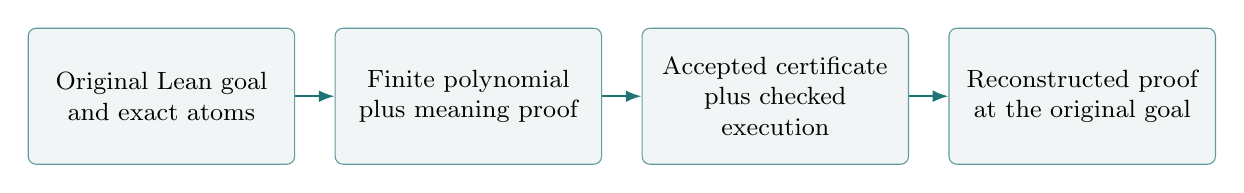
\begin{tikzpicture}[
 node distance=5mm,
 box/.style={draw=accent!70,fill=pale,rounded corners=1mm,
 text width=1.24in,minimum height=.68in,align=center,font=\small},
 arr/.style={-{Latex[length=2mm]},thick,draw=accent}]
\node[box] (a) {Original Lean goal\\and exact atoms};
\node[box,right=of a] (b) {Finite polynomial\\plus meaning proof};
\node[box,right=of b] (c) {Accepted certificate\\plus checked execution};
\node[box,right=of c] (d) {Reconstructed proof\\at the original goal};
\draw[arr] (a)--(b);\draw[arr] (b)--(c);\draw[arr] (c)--(d);
\end{tikzpicture}
\end{center}

The supplied Python companion implements the finite polynomial operations and
checks illustrative certificates. That execution is a sanity check of the
reference algorithm, not a Lean proof of Theorem~\ref{thm:polycheck} or a
verified reifier. The supplied small Lean model addresses refinement and
behavioral composition, not this full polynomial development. The remaining
formalization work is explicitly recorded in Section~\ref{sec:implementation}.

\subsection{Where existing tactics belong}
The first production implementation should call existing proof-producing
Lean arithmetic tactics before building a competing discovery engine. The
round-two toolchain probes already exercised \code{linear_combination} and
\code{grobner}; their reported measurements concern a particular old pin and
small certificate family, not this proposal's runtime \cite{syn,workbenches}.
Current Lean documentation describes \code{grind} as cooperating proof-producing
reasoning components, including polynomial reasoning \cite{leangrind}.

For \Karst, a successful invocation is one provider returning a checked proof
of the original target. Its failure means only that this route did not solve
the request under its limits. No external reusable certificate format should
be assumed without an actual adapter. The retained proof term is already
valid evidence for replay in its pinned environment.

The independent polynomial-certificate route earns its place only if it adds
something measurable: a compact service-independent artifact, a domain not
served by existing tactics, better checking costs on an actual workload, or a
useful interface to an external producer. Reimplementing existing arithmetic
under a new language name is not itself a contribution.

\section{Typed observations: backward precision and forward proof}\label{sec:jets}

\subsection{An observation is not a refinement of the representation's identity}
For $\Delta\in R[[t]]$, define
\[
 \operatorname{Jet}(\Delta,N)
   :=\{J\in R[t]\mid\forall k<N,\ [t^k]J=[t^k]\Delta\}.
\]
This notation describes a value $J$ together with a relation to the fixed
$\Delta$. It does not identify the polynomial $J$ with the full series. The
view of $\Delta$ records that this observation is available; the representation
$J$ remains a different object.

The source-level type system has two useful operations: weaken an observation
to a lower precision, and satisfy a requested observation by a theorem with
known input requirements. These are applications of proved implications, not
subtyping between the underlying polynomial and power-series types.

\subsection{The residual bridge, inherited and made operational}
The following is the central formal-root theorem emphasized by Locus and
adopted by both syntheses \cite{syn,workbenches}.

\begin{proposition}[Residual identification of an existing root]\label{prop:residual}
Let $F(Y)\in R[[t]][Y]$ over a commutative ring $R$, and suppose
$F(\Delta)=0$ with $\Delta(0)=d$. Let $\overline F\in R[Y]$ be obtained by
taking constant coefficients. Assume $\overline F'(d)$ is a unit. If $N\ge1$,
$J(0)=d$, and $F(J)$ has zero coefficients below $N$, then
$J\equiv\Delta\pmod{t^N}$.
\end{proposition}
\begin{proof}
Polynomial subtraction factors as
$F(J)-F(\Delta)=(J-\Delta)U$ for a formal series $U$.
Its constant term is $\overline F'(d)$ because $J$ and $\Delta$ have the same
constant term. Hence $U$ is invertible. Multiplication by $U^{-1}$ shows that
$J-\Delta$ belongs to the ideal $(t^N)$.
\end{proof}

The theorem concerns an already fixed root. It neither constructs that root
nor replaces it by a canonical solution. The unit hypothesis and shared
constant coefficient are mathematical premises, not metadata. In $\Z/4\Z$,
$F(Y)=2Y$, $\Delta=0$, and $J=2t$ have zero residual and nonzero derivative
but do not agree below degree two. A candidate for the wrong root of
$Y^2-1$ can have zero residual and unit derivative while failing the selected
constant term. Both failures must be diagnosed at the contract boundary.

\subsection{A concrete backward-demand example}
Suppose an arbitrary rational formal series $\Delta$ is given by
\[
 \Delta^2=1+t,\qquad \Delta(0)=1.
\]
The task is to obtain the coefficients of its \emph{formal derivative} below
degree four. Differentiation gives the coefficient relation
\[
 [t^k]\Delta'=(k+1)[t^{k+1}]\Delta.
\]
A sufficient input is therefore a jet of $\Delta$ below degree five. The
planner should request that precision before calling the producer.

The polynomial
\[
 J=1+\frac12t-\frac18t^2+\frac1{16}t^3-\frac5{128}t^4
\]
has constant term one and residual $J^2-(1+t)$ vanishing below degree five.
The reduced derivative of $Y^2-(1+t)$ at one is the unit $2\in\Q$.
Proposition~\ref{prop:residual} identifies $J$ as the requested observation of
this $\Delta$. Differentiation then yields
\[
 \Delta'\equiv
 \frac12-\frac14t+\frac3{16}t^2-\frac5{32}t^3
 \pmod{t^4}.
\]

\begin{lstlisting}[caption={A demand-driven observation with no object substitution.}]
given Delta : PowerSeries Rational
  with Delta^2 = 1 + t and constant Delta = 1

request derivative Delta as jet below 4
  using formal_derivative
-- generated demand: a jet of this Delta below 5
-- producer: polynomial J
-- checks: constant, residual, unit derivative
-- output: derivative J, certified below 4
\end{lstlisting}

The requested precision remains fixed. Returning a derivative jet below degree
three is a weaker result and cannot close this request. Returning the exact
derivative of the polynomial $J$ is also not, by itself, a statement about
$\Delta$. The bridge theorem is what connects them.

This is not an analytic Taylor remainder estimate. No convergence radius,
real or complex branch of an analytic square root, or numerical error bound
has been established. A later analytic request must provide a realization and
convergence theorem. The formal derivative annotation prevents the language
from silently importing that stronger interpretation.

\subsection{The same mechanism handles domains, not just precision}
A transformation known on a larger domain can answer an equality request on a
smaller domain after proving the inclusion. The reverse direction requires
new evidence. A solver returning a witness for $ax=b$ when $a\ne0$ cannot
answer a request for the complete solution predicate for all $a,b$.
The singular branches remain part of the specification:
\[
 a\ne0:\{b/a\},\qquad
 a=0=b:\text{all elements},\qquad
 a=0\ne b:\varnothing.
\]
These examples, inherited from the second round, illustrate why observation
precision, domains, and completeness should be predicates in the typing
request rather than informal output labels.

There is no single ordering covering all guarantees. The inference engine
uses the actual implication theorem needed by each consumer. Its planner may
choose sufficient requirements rather than weakest ones, but it must report
when a selected route asks for a stronger hypothesis than the statement gives.

\section{Leant integration: from candidate types to intended behavior}\label{sec:leant}

\subsection{Preserve the authority boundaries already present}
In the inspected \code{Verification.hs}, \code{Verified candidate} is an
opaque receipt of callback acceptance; its documentation explicitly says that
it is not a kernel proof, solver certificate, or behavioral proof. The verifier
retains the actual accepted rendering and keeps quota and failed-group
accounting separate \cite{verify}.

In \code{PostVerification.hs}, a fresh rank-two epoch scopes occurrence
handles. A proposed reorder must be an exact bounded permutation of the
original accepted occurrences; omission, duplication, and out-of-range indices
are rejected. The constructor and index are private, and the original receipt
is selected rather than trusting a reassociated payload \cite{postverify}.
This is valuable precedent for \Karst's exact request and evidence identity.

The length-ranking documentation further distinguishes stable ranking from
explicitly authorized hard filtering. Its current finite list-spine dialect
uses a canonical arithmetic query and independently replays reported
counterexamples in the vendored engine. It explicitly lists broader
counterexample-guided synthesis and Lean-checked proof artifacts among the
remaining proposed work \cite{length}.

The integration should reuse these boundaries. It should not promote an
opaque operational receipt to a theorem just because its Haskell constructor
is inaccessible to ordinary callers.

\subsection{A two-stage synthesis contract}
A \Karst\ construction request has the logical result type
\[
  \{x:A\mid\Spec(x)\},
\]
where both $A$ and $\Spec$ are fixed at the original Lean telescope. A provider
may first search for a candidate $x:A$ and then search for a proof of
$\Spec(x)$. Alternatively, it may synthesize them together. In either case,
acceptance requires both.

For proof-only obligations, $A$ itself may be a proposition and the returned
term its proof. For data construction, the distinction between inhabiting the
base type and satisfying the behavioral refinement is essential. A suggested
sorting function is not accepted as a sorter merely because Lean checks its
list-to-list type.

The exact selected candidate should be preserved through every rendering and
behavioral pass. If a candidate is wrapped, optimized, or reconstructed as a
new expression, its behavioral evidence must be transported by a theorem
about that transformation or recomputed for the new expression. Textual
similarity is not an identity proof.

\subsection{A new bridge test: abstract counterexamples must be realizable}\label{sec:empty}
Length observations reveal a subtle boundary that matters when mathematical
refinements enter the type system. Consider
\[
 \operatorname{dropAll}:\operatorname{List}(\operatorname{Empty})
      \to\operatorname{List}(\operatorname{Empty}),
 \qquad \operatorname{dropAll}(xs)=[].
\]
Every list of an empty type is empty, so this function preserves length on
\emph{every actual input}. An abstraction that admits arbitrary natural input
lengths can produce the apparent counterexample ``input length one, output
length zero''. There is no corresponding input list.

This is a stress test for a \emph{future original-Lean behavioral bridge}, not
an allegation that the inspected Leant implementation accepts this target or
mishandles it. It demonstrates why replay inside an abstract behavior model,
even when exact for that model, does not alone establish a negation of an
arbitrary original Lean statement.

A valid original-target refutation needs a realizable input satisfying the
original input refinements, together with checked evaluation or reasoning that
it violates the postcondition. Schematically, the required witness has type
\[
 \exists x:A,\ P(x)\land\neg Q(x,f(x)).
\]
When the input telescope is dependent, the whole tuple must be realizable;
independent assignments to each abstract component may violate its shared
constraints. A polymorphic request can sometimes be refuted by choosing an
inhabited type such as \code{Unit}, but that is a different quantifier structure
from a request fixed at \code{Empty}.

The same problem occurs beyond lists. A finite jet may satisfy algebraic
constraints without being an observation of the selected analytic object;
a proposed matrix dimension may be inconsistent with a refined index type;
a countermodel to a relaxed equation may violate the original nonzero guards.
The type system's job is to keep that admissibility information attached to
the request.

\subsection{The obligations on which Leant should be measured}
The first integration experiment should collect actual generated obligations,
not a convenient unrelated synthesis benchmark. The finite-map example yields
composition of injectivity proofs, transport through displayed inverse maps,
and restricted-map well-definedness. The exact-quotient example yields
composition of parity, divisibility, and cast lemmas. The jet workflow yields
assembly of a residual theorem, a unit proof, and precision weakening.

Some are single-lemma retrieval; others require composing several constructors
or theorem applications. Record those classes separately, compare against the
same selected library and existing Lean automation, and retain failures.
A sophisticated synthesizer is not necessarily the best tool for every one of
these small obligations. Its value should be demonstrated rather than inferred
from the appeal of structural synthesis.

\subsection{Tactic suggestions need a source-edit receipt too}
A candidate term checked at the right type and a tactic edit that works in the
actual source are separate deliverables. The edit must be inserted into a
transactional snapshot of its origin, elaborated with the surrounding syntax
and name resolution, and checked for completion of the intended root goal.
Failed attempts restore both source and elaborator state.

A reduction in the number of visible goals is local progress, not theorem
completion. An accepted proof term does not make a malformed displayed edit
correct. A successfully replayed edit does not excuse a changed theorem
statement. These requirements extend the source-level acceptance contract;
this article does not claim the complete editor integration already exists.

\section{Should Lean's kernel type system change?}\label{sec:kernel}

\subsection{The serious alternatives}
A library-only approach can already provide the semantic contracts in this
article. It has the lowest compatibility risk and is the first baseline.
A native Lean elaborator extension can add refined declarations, property
requests, typed observation commands, and source-to-proof records while
emitting ordinary Lean terms. This is the recommended route.

A new primitive refinement constructor in the kernel could make the surface
more uniform, but its logical content is already represented by predicates
and subtypes. It would need a compelling advantage in elaboration behavior,
proof size, or metaprogramming interfaces, demonstrated against the conservative
encoding. The existence of long proofs alone does not establish such an
advantage.

A more radical option would let propositional equalities or solver-derived
constraints participate directly in kernel conversion. That changes the
trusted implementation boundary and the interaction between proof search and
type checking. Even when a narrowly specified extension could be justified,
there is no need to make arbitrary CAS normalization or refinement entailment
part of conversion to obtain the benefits proposed here. A checked equality
can instead justify an explicit transport term.

This distinction matters for dependent indices. A vector indexed by $n+1$
and one indexed by $1+n$ can be related by a proved equality of indices.
The author may reasonably expect that transport to be automated. The
implementation can generate it without pretending that all mathematically
equal indices are definitionally identical. The resulting explicit transport
can be retained and inspected when an index expression changes.

\subsection{A refined domain is not merely a precondition}
One subtlety deserves an explicit semantic decision. The expressions
\[
 f:A\to B\ \text{with}\ \operatorname{Beh}(P,Q,f)
 \quad\text{and}\quad
 g:\{x:A\mid P(x)\}\to B
\]
are not the same interface. The first contains a total underlying function on
$A$, with guarantees only on the specified inputs. The second is defined only
on the refined domain; extending it to all of $A$ requires additional data or
principles and may be impossible when $B$ is empty.

\Karst\ therefore uses \code{with} for a behavioral view of an already typed
function and explicit refined-domain syntax for a restricted function. It
never treats a precondition proof as an automatic license to enlarge the
function's domain. This prevents a source-level refinement convenience from
silently changing the mathematical object.

For compatibility, ordinary Lean expressions retain ordinary Lean semantics
by default, including its total operations. A partial-expression package is
explicit. An imported total expression is not silently reinterpreted as a
partial one merely because its usual informal presentation has a pole. This
is a default for interoperability, not a claim that total semantics is always
the most readable choice.

\subsection{What native support would actually help}
The first native extensions worth considering are elaborator and editor APIs:
stable access to local expression identity, typed requests that distinguish
data holes from proof holes, structured provenance for inserted transports,
and reliable transactional replay of a displayed edit. None requires a new
axiom or a new logical connective.

The existing coercion mechanism already inserts designated functions when an
expected type differs from an inferred one \cite{leancoercions}. A
refinement-aware layer can cooperate with that mechanism, but must record
when it changes the underlying object versus when it supplies only a proof.
A field coercion and a proof of nonzeroness are not the same kind of inference.

F* supplies a useful comparison: it makes refinement and effectful
specification central to proof-oriented programming \cite{fstarintro,fstarref}.
\Karst's proposed niche is not a more expressive logic. It is a Lean-native
mathematical authoring workflow that preserves existing objects, libraries,
and proof evidence while making local properties usable as source-level types.
Whether that niche warrants a separate surface is an empirical question.

\section{Editing, explanations, and collaborative proof development}\label{sec:editing}

\subsection{Diagnostics should expose the missing mathematical distinction}
A failed refinement request should show the property required by the operation,
the closest available evidence, and the precise missing bridge. For example:
\begin{lstlisting}[caption={A proposed diagnostic, not output of an implemented tool.}]
Cannot invert this integer coefficient.
Required: IsUnit (2 : Int)
Available: 2 != 0; multiplication by 2 is injective
These facts permit cancellation, not an inverse in Int.
The original coefficient domain has not been changed.
\end{lstlisting}

Or, for the finite-map construction:
\begin{lstlisting}[caption={A domain-preservation diagnostic.}]
Cannot construct kZ : Z -> Z yet.
Required: for every i != 0, k i != 0
Available: injective k
Missing on the selected route: k 0 = 0
The restriction remains an open definition obligation.
\end{lstlisting}

The second message does not prove that no restriction exists. It states why
the selected routine route is incomplete. Another proof of domain preservation
would also suffice. The distinction between a sufficient rule and a necessary
condition is crucial to honest diagnostics.

\subsection{A document has more obligations than its last theorem}
Every displayed formal assertion must have checked evidence, even when the
final theorem can be proved without it. Otherwise a document could contain a
false intermediate assertion and still receive a misleading overall success
mark. A parser must also distinguish a quoted conjecture, an open obligation,
and an asserted theorem.

For conditional results, the display should separately report: the checked
conditional theorem, which guards have been discharged in the current scope,
and whether the original request is complete. For example, a checked proof of
$G\to Q$ with $G$ still open is useful progress but is not a checked proof of
$Q$ in that context.

The selected method is another dimension. A command explicitly requesting
reindexing should not be reported as a successful reindexing step when its
coverage condition failed and an unrelated theorem closed the goal. An open
\code{infer} request can accept any permitted proof of the fixed property;
a named \code{using} request retains its advertised theorem or method skeleton.
The source can deliberately change the method, but that change should be visible.

\subsection{Merging refinements versus merging objects}
Two collaborators may prove different properties of the same unchanged
object. Their evidence records can be merged after each proof is checked in
the destination environment and its dependencies are available. They need not
agree on an identical proof term.

If they choose different witnesses, even witnesses satisfying the same
existential specification, the merge is not automatically a merge of two
properties of one object. It needs a selected witness, an equality or
observational bridge sufficient for the consumers, or separate named objects.
Likewise, choosing different ring structures or different root branches is a
semantic conflict, not a textual conflict that a property union resolves.

The first collaboration experiment should be small: two branches refine the
same map independently; a second pair changes its defining term; a third pair
selects different representation routes. Measure how often ordinary Lean
rechecking resolves the merge and where additional provenance improves the
explanation. A universal semantic merge algorithm is not a prerequisite.

\subsection{Replay and upgrades}
Retained evidence is authoritative only relative to the recorded environment
and acceptance policy. A library or toolchain upgrade creates a new validation
attempt. Reconstruct the target and evidence in the destination environment,
check the original mathematical guarantee, inspect the actual dependency
inventory, and emit a new receipt.

A changed native-evaluation axiom naming scheme must not be handled by merely
renaming an allowlist. Policy classifies the intended trust assumptions and
checks their concrete realization in that environment. Similarly, an unchanged
printed theorem with a changed instance interpretation is a semantic change.
A content hash is useful for detecting change; it is not a theorem that the
changed object has the old meaning.

\section{Implementation plan with explicit stopping points}\label{sec:implementation}

The complete language described above is a research design, not a committed
implementation. To avoid another round of expanding architecture without
feedback, the implementation should be divided into a few independently useful
artifacts.

\subsection{First: host-native contracts and one sound computational slice}
Start with ordinary Lean definitions for a view, behavior, exact observation,
and evidence request. The accompanying \code{KarstCore.lean} illustrates some
of these definitions and their elementary theorem constructors. It uses no
proposed \Karst\ commands, but it has not been compiled here. Its first use
must be compilation and axiom auditing, not publication as an already verified
library.

The first computational slice should formalize the sparse integer polynomial
representation from Section~\ref{sec:cas}. Deliverables are the parser's
well-formedness boundary, denotation, normalization and operation lemmas,
Theorem~\ref{thm:polycheck}, actual checked evaluation, and a reifier for a
small original Lean goal language. A useful acceptance example is a
multivariate consequence with two hypotheses, accompanied by a corrupted
multiplier, arity mismatch, and stale atom mapping.

This directly answers the syntheses' request for a sound checker. The paper
proof and executed Python reference model supplied here clarify the intended
formalization, but do not complete that Lean deliverable. Existing arithmetic
tactics must be included as controls from the beginning.

\subsection{Second: a deliberately small refinement engine}
Implement a local fact index and a small theorem registry for the finite-map
example. Restrict automatic rules to checked projections, involution-to-
injectivity, composition, map-into proofs, and the selected equivalence
transport wrappers. Reuse Lean's local context rather than mirroring it into a
second semantic database.

At this stage use ordinary Lean syntax plus explicit commands requesting a
property. If the registry adds no value beyond a small collection of existing
\code{have} statements and tactics, retain those library improvements and stop.
A new language is not required for success.

The next package may expose exact quotient contracts and the residual-jet
bridge, but only after the first index can explain its generated obligations
and invalidate them correctly under edits. General equality saturation,
weakest-domain inference, global coercion search, and a universal property
ontology are outside this first engine.

\subsection{Third: one Leant behavioral proof bridge}
Use Leant to generate a fixed candidate at a fixed Lean type, then require one
universal behavioral theorem in a small supported family. The first candidate
family should make a structural false positive easy to construct, such as
list length preservation versus a permutation requirement.

Keep the existing length ranking/filtering as discovery assistance. Add an
explicit adequacy and realizability boundary before any abstract outcome is
published as original-target logical evidence. Include the \code{List Empty}
case as a specification stress test, whether or not it belongs to the initial
provider's eligible fragment. Unsupported inputs should be reported as such,
not silently coerced into a broader model.

\subsection{Only then: the mathematical surface}
Add the small grammar once the same semantic records work with ordinary Lean.
The new frontend and the Lean frontend should emit the same request objects
and consume the same evidence. A read-only mathematical document view can be
built independently and may turn out to be the more valuable artifact.

A sensible stopping rule is substantive: stop expanding syntax when its only
benefit is hiding work already hidden by the shared library, when semantic
reading becomes less accurate, or when users spend more time repairing opaque
inference than writing explicit proofs. Continue only when a specific source
construct demonstrably improves the authoring task.

\section{Evaluation: measure the source-level contribution}\label{sec:evaluation}

\subsection{A shared-library comparison with a refinement ablation}
The inspection examples are development material. Once examined here, neither
the finite-map file nor the Frey-package assembly is a sealed holdout. The
shared binomial, Abel, and derivative examples from earlier rounds are controls,
not independent new evaluation tasks \cite{syn,workbenches}.

A fair comparison has five nested conditions:
\begin{center}\small
\begin{tabularx}{\textwidth}{@{}P{.45in}Y@{}}
\toprule
Arm & Available infrastructure\\
\midrule
$L_0$ & Ordinary Lean and its existing library and automation.\\
$L_1$ & $L_0$ plus every theorem wrapper, definition package, and checker built
for this project.\\
$L_2$ & $L_1$ plus the same providers, budgets, and retained-evidence services.\\
$L_3$ & $L_2$ plus the property index and refinement inference, still with an
ordinary Lean frontend.\\
$L_4$ & The same infrastructure with the proposed mathematical surface.\\
\bottomrule
\end{tabularx}
\end{center}
The distinction between $L_2$ and $L_3$ measures the refinement machinery;
between $L_3$ and $L_4$ it measures the new surface. Infrastructure costs must
be charged to the project and amortized over observed reuse, not hidden in an
unlimited collection of new magic lemmas.

Measure authoring and repair time, number and kind of interventions, success
within a fixed budget, checker time, retained artifact size, and semantic
reading accuracy. Count both proof configuration and mathematical code, but
report them separately. Use paired tasks and counterbalanced ordering so that
learning the mathematics in the first condition does not become an apparent
language advantage in the second.

\subsection{A semantic-reading test}
Before showing expanded evidence, ask readers to identify the actual carrier,
input domain, quantified dependencies, selected object, branch, precision,
completeness guarantee, and open assumptions. Include equally polished compact
renderings whose underlying guarantees differ. Then reveal the expanded view
and measure whether it corrects misunderstandings.

For this proposal the most informative pairs are: proposition-valued finiteness
versus an executable enumeration; a total function with a precondition versus
a restricted-domain function; a length-preserving function versus a sorter;
and a polynomial derivative versus a derivative observation of an existing
formal root. A shorter proof display that systematically confuses these pairs
is not an improvement.

\subsection{A prototype test register, not a claimed passed suite}
Table~\ref{tab:mutations} lists required paired acceptance tests for a Lean
prototype. These have \emph{not} been executed as \Karst\ tests. The Python
companion covers selected finite arithmetic and synthetic metadata neighbors
only. The larger fifty-one-family register in the second-round synthesis remains
useful and should not be declared passed by these small experiments.

\small
\begin{longtable}{@{}P{.35in}P{2.60in}P{3.05in}@{}}
\caption{Paired prototype tests: every rejection must have an accepted neighbor.}\label{tab:mutations}\\
\toprule
Id & Negative mutation & Required positive neighbor or response\\
\midrule
\endfirsthead
\toprule Id & Negative mutation & Required positive neighbor or response\\\midrule
\endhead
T1 & Reuse a property of another local variable with the same printed name.
& The exact original variable succeeds; a different anchor requires a proved bridge.\\
T2 & Reuse a fact after changing the selected algebra structure.
& The unchanged structure succeeds; a checked structure transport is explicit.\\
T3 & Move branch-local nonzeroness into a sibling branch.
& Use inside its branch succeeds; an exported conditional theorem stays conditional.\\
T4 & Extract executable enumeration from proposition-valued finiteness alone.
& The proposition-level finite-map theorem succeeds; explicit enumeration data supports execution.\\
T5 & Accept reversal as sorting because its length is correct.
& A candidate with permutation and orderedness proofs succeeds.\\
T6 & Refute a \code{List Empty} contract using an unrealizable nonzero length.
& A typed concrete counterexample on an inhabited domain can be accepted with its proof.\\
T7 & Extend a function on a refined domain to the whole carrier without data.
& Restriction of an existing total function succeeds with its map-into proof.\\
T8 & Restrict an injective map to nonzero elements without a preservation proof.
& The fixed-zero argument supplies preservation; another direct proof is also accepted.\\
T9 & Treat a nonzero or regular integer as a unit.
& Cancellation uses regularity; inversion succeeds only with unit evidence.\\
T10 & Cast an inexact integer quotient as a rational quotient.
& The exact-divisibility and nonzero-denominator case succeeds.\\
T11 & Keep input jet precision after differentiation.
& One additional input coefficient satisfies the stated sufficient contract.\\
T12 & Return the wrong formal root branch with a correct residual.
& The selected constant coefficient and unit condition give the valid observation.\\
T13 & Supply malformed certificate arities or monomial dimensions.
& A well-formed certificate with the same intended consequence succeeds.\\
T14 & Replace the checker execution proof by a native byte-string assertion.
& Checked reduction or another policy-approved evidence route succeeds.\\
T15 & Reify an opaque atom under the wrong valuation.
& Exact original-expression meaning proofs permit reconstruction.\\
T16 & Use the desired result to justify its own guard.
& An acyclic proof graph from actual premises succeeds; explicit induction uses a checked rule.\\
T17 & Publish an unused false formal assertion beside a valid final proof.
& Every asserted node has a proof, or is explicitly marked as an open conjecture.\\
T18 & Replay an edit against a different source origin or count progress as completion.
& Exact-origin transactional replay and the final root check both succeed.\\
\bottomrule
\end{longtable}
\normalsize

\section{Decisions returned to the two syntheses}\label{sec:decisions}

The two reports ask overlapping questions rather than prescribing a finished
protocol. The following decisions make this proposal falsifiable and avoid
presenting an open design choice as a measured answer.

\small
\begin{longtable}{@{}P{.32in}P{1.60in}P{4.05in}@{}}
\toprule
& \emph{Nine Workbenches} question & Decision in this proposal\\
\midrule
\endfirsthead
\toprule & Question & Decision\\\midrule
\endhead
R1 & How is a checker proved sound? & Section~\ref{sec:cas} specifies integer
sparse monomials, denotation, normalization, operation lemmas, arity checking,
and target reification. The paper proof is complete for that contract; the
Lean checker and reifier remain implementation work.\\
R2 & Where does \code{grobner} sit? & A bounded proof-producing provider and
control, not a negative oracle. Retain its resulting proof; assume no exported
certificate API not actually supplied by an adapter.\\
R3 & What is new workspace state? & Only source identity, property-role
indexing, support/provenance, observation links, and acceptance records.
Ordinary contexts, terms, instances, and proof checking remain Lean's.\\
R4 & Partial or total default? & Preserve ordinary Lean semantics when lifting
existing source. Restricted-domain functions and partial-expression packages
are explicit; preconditions do not silently change a function's domain.\\
R5 & Which package first? & One polynomial checker first for the computational
boundary; a small finite-map refinement package for the type-layer experiment.
Other packages follow measured demand. Inspected Bell/Abel examples are not
sealed holdouts.\\
R6 & When use acceleration? & No numeric threshold is claimed. Measure balanced
and sparse multivariate inputs, large coefficients, and proof reconstruction
under the actual target toolchain before adopting one.\\
R7 & How survive upgrades? & Revalidate in the destination environment and
policy; inspect actual axiom dependencies and emit a new receipt.\\
R8 & What does Leant contribute? & Measure compositions from finite-map,
exact-quotient, and jet assembly obligations separately from single-lemma
retrieval. Require original-target behavioral evidence.\\
R9 & Can mutations execute? & A finite companion is executed here; the full
Lean register is not. Table~\ref{tab:mutations} gives paired obligations for the
prototype rather than an inflated pass count.\\
R10 & Another design or a prototype? & This requested article supplies the
specified type discipline, a small uncompiled Lean semantic model, and an
executed Python reference. Its implementation gate remains a compiled,
end-to-end evidence slice, not a larger grammar.\\
\bottomrule
\end{longtable}
\normalsize

The parallel synthesis's additional choices are settled as follows. Authors may
delegate witness construction by an unchanged explicit specification, but not
replacement of a previously quantified object. Every unresolved domain,
branch, precision, completeness, or trust condition stays visible. Automatic
representation changes use registered relation-specific theorems and retain the
selected route; arbitrary global planning is deferred. Result guarantees are
ordinary Lean predicates with an extensible vocabulary, not a fixed confidence
ladder. Negative provider outcomes remain operational unless original-target
negative evidence is checked. Publication stores the accepted object, statement,
proof or certificate, context, and policy, while discovery logs are optional.
A library, an index, or a read-only document view is a legitimate stopping
point.

\section{What has been established, and what has not}\label{sec:status}

The semantic rules in Sections~\ref{sec:semantics} and~\ref{sec:behavior}, the
finite restriction and transport arguments, the Frey divisibility argument,
and the polynomial checker theorem have explicit paper proofs. The residual
bridge is inherited from the earlier proposals and restated with its required
premises. The architecture is a proposal about how to implement these rules,
not an already validated proof environment.

The executed companion produced the following results. The counts use different
units and should not be summed into a language-validation score.
\begin{center}\small
\begin{tabularx}{\textwidth}{@{}Y r Y@{}}
\toprule
Check group & Cases & What was actually checked\\
\midrule
Finite endomaps & 3,414 & All maps on sizes zero through five; 154 injective
maps satisfy the finite normalization/restriction checks.\\
Polynomial protocol neighbors & 7 & Valid and malformed small certificates.\\
Polynomial denotation samples & 720 & Seeded checks of operations over integers,
$\Z/4\Z$, and $\Z/5\Z$ in one to three variables.\\
Sorting samples & 364 & All lists of length at most five over three values,
with explicit weaker-behavior counterexamples.\\
Length realizability & 1 & The empty-type input-domain distinction.\\
Exact quotient samples & 312 & The congruence/parity denominator claims, not
Fermat's Last Theorem or a curve comparison theorem.\\
Formal jet neighbors & 5 & Rational residual, derivative coefficients, branch,
precision, and nonregular-element examples.\\
Synthetic origin/scope tests & 11 & A metadata model of identity, scope, and
acyclic dependencies; not a Lean context checker.\\
\bottomrule
\end{tabularx}
\end{center}

No Lean executable was available in this session. Consequently
\code{examples/KarstCore.lean} is supplied as uncompiled source, its audit
commands have not produced an inventory, and no proof in this article is
called machine-verified on the basis of that file. The companion is standard
Python and was executed; its output and limitations are retained in
\code{evidence/results.json} and \code{evidence/run.log}.

The main unresolved risks are practical: whether the fact index offers enough
benefit over current Lean automation, whether its dependency explanations are
readable, whether property search remains predictable, whether useful behavioral
bridges can be proved without excessive adapter cost, and whether the surface
helps authors rather than only making completed proofs look attractive.
These are implementation and evaluation questions, not gaps that can be
closed by choosing a more ambitious language name.

\section{Conclusion}
The third round should move from ``a computation returns an answer with a
proof'' to ``a mathematical object has exactly these usable properties here,
and this operation demands exactly this behavior.'' That is the role proposed
for \Karst's source-level type system.

The central design principle is simple: \emph{refine knowledge without silently
changing the object}. Around it, a disciplined elaborator can supply ordinary
proofs of injectivity, domain preservation, divisibility, precision bounds, and
behavioral consequences. It can help Lean understand a mathematician's
compression without turning that compression into an uncheckable assumption.

The strongest evidence in favor of the approach is structural, not yet
empirical. The finite-map proof contains repeated property transport that a
small theorem registry can plausibly expose. The Frey package demonstrates
that mathematical properties already belong naturally in Lean interfaces,
while its compact assembly proof warns against overstated savings. Leant
supplies concrete machinery for candidate identity and behavioral exploration,
but the empty-type example shows why original semantics and realizability
must accompany any stronger logical claim.

The recommended result is therefore an incremental Lean extension with a
small, checkable semantic core. Kernel changes are not ruled out forever;
they simply have not earned their cost here. A successful implementation may
be a new mathematical frontend, or it may be a better Lean library, property
index, and document view. Either is worthwhile if it lets the human write the
mathematical argument while preserving the exact statement, objects, and
evidence that make the argument a proof.

\appendix
\section{Minimal grammar and lowering conventions}\label{app:grammar}

The following grammar is illustrative rather than a parser specification.
It shows the intended small boundary; expressions and propositions are hosted
Lean syntax after the surrounding binders have been resolved.
\begin{lstlisting}
statement ::= theorem name ":" telescope "show" proposition proof
            | define name ":" type contract implementation

telescope ::= ("given" binder ("with" properties)?)*
properties ::= proposition ("," proposition)*
contract ::= ("ensures" proposition)*

step ::= "let" binder ":=" expression
       | "establish" proposition "by" proof
       | "infer" proposition ("using" method)?
       | "choose" binder "with" proposition ("using" method)?
       | "construct" binder "satisfying" proposition
       | "observe" binder ":" observation "using" method
       | "restrict" expression "to" domain "as" binder proof
       | "transport" expression "along" expression "as" binder
       | "under" proposition ":" block
       | "induct" expression ":" cases
       | "conclude" proposition "by" proof
       | lean_block
\end{lstlisting}

A \code{given} refinement lowers to explicit theorem parameters. An
\code{establish} or \code{infer} refinement lowers to a theorem about the
existing expression. A \code{construct} request lowers to a value plus a
specification proof, respecting the declared computability policy. An
\code{observe} request lowers to a representation plus a relation to its
fixed subject. A \code{restrict} or \code{transport} command creates a new
object with an explicit connecting theorem. An \code{under} block introduces
an assumption only in that block and abstracts it when leaving.

A rule package should specify: its checked theorem constant; the input and
output roles in that theorem's telescope; whether it only supplies proof or
also chooses data; the exact relation it establishes; and its local search
policy. Only the first four affect the logical assembly. Budgets and priorities
affect discovery, not the meaning of the theorem.

\section{Source register and reading scope}\label{app:sources}

Repository revisions were resolved during this review. The full commit IDs
below identify the intended snapshots; bibliography links use them rather
than mutable branch names. Blob IDs in the accompanying JSON register identify
selected inspected files. No repository-wide build or claim about every file
at those revisions follows from this source inspection.

\begin{center}\small
\begin{tabularx}{\textwidth}{@{}P{1.15in}Y@{}}
\toprule
Repository & Revision and inspected scope\\
\midrule
Brainstorm & \code{b052ec011beb96a7c48df2a9988823f0f779b445}. Both second-round
synthesis TeX reports, including their substantive comparisons, mathematical
bridges, experiments, corrections, and third-round questions. The nine
individual proposals are discussed through those syntheses; their entire
source trees were not independently audited.\\
ProveIt & \code{24ce8bd743eaab64a91ce90725ea00f498d319d2}.
The complete \code{NoFiniteModel/FiniteTypes.lean} and
\code{NoFiniteModel/Theorem.lean} source files.\\
Fermat's Last Theorem & \code{aa2d8b34692b16c70f699536de0d8e75b9a3e9ef}.
Frey-package definitions, the final solution's mathematical body and extensive
configuration prelude, and the proof-path document. Large configuration
responses were inspected in ranges; this is not a complete audit of every
listed attribute or imported theorem.\\
Leant & \code{3a40904be8a410d832d9ab6900b3d3e7b425eccb}.
\code{Verification.hs}, \code{PostVerification.hs}, the behavioral-length
documentation's opening authority and status sections, and portions of the
synthesis-internals documentation.\\
\bottomrule
\end{tabularx}
\end{center}

The two reports are read as revised documents. Historical timings and theorem
availability probes remain observations of their stated environments, not new
measurements performed for this article. In particular, this article neither
reuses those numbers as current benchmarks nor calls their unverified checker
a completed proof-producing CAS.

The official Lean reference pages were consulted on 6 September 2026; the
\code{latest} reference identified itself as version \code{4.34.0-rc2}.
That documentation version is not an executed toolchain for this package.
The current F* tutorial was used only as primary-source context for refinement
and proof-oriented programming, not as evidence for the performance or
soundness of the proposed integration.

\section{Files and reproducibility}\label{app:repro}
The archive contains the self-contained \code{karst.tex}, its rendered
\code{karst.pdf}, build instructions, a source register, the uncompiled
\code{examples/KarstCore.lean}, and the executed Python companion with its
result file and log. No font files, downloaded repository snapshots, or
third-party reports are redistributed.

To reproduce the finite checks, run:
\begin{lstlisting}
python3 evidence/companion.py
\end{lstlisting}
The random samples use seed \code{20260906}; the remaining cases are deterministic
or exhaustive over their stated finite inputs. Running the script rewrites
\code{evidence/results.json}. It requires only Python's standard library.

To build the article, run:
\begin{lstlisting}
latexmk -pdf -interaction=nonstopmode -halt-on-error karst.tex
\end{lstlisting}
The bibliography is embedded and the diagram is drawn in TeX; no network
access is needed. A separate pinned Lean installation is needed to check the
Lean model. Its final \code{\#print axioms} commands are an audit request, not
an already recorded result.

\clearpage
\begin{thebibliography}{99}
\small

\bibitem{syn}
\emph{Mathematical Objects, Certified Computation: A Unified Evaluation of
Nine Second-Round Proof-Language Proposals}. Brainstorm, revised synthesis,
6 September 2026.\par
\url{https://github.com/VladimirReshetnikov/Brainstorm/blob/b052ec011beb96a7c48df2a9988823f0f779b445/docs/round-2/synthesis/unified-report.tex}

\bibitem{workbenches}
\emph{Nine Workbenches: A Unified Review of the Second-Round Proof-Language
Proposals}. Brainstorm, revised report incorporating parallel-review
corrections, September 2026.\par
\url{https://github.com/VladimirReshetnikov/Brainstorm/blob/b052ec011beb96a7c48df2a9988823f0f779b445/docs/round-2/unified_report/unified_report.tex}

\bibitem{finite}
Vladimir Reshetnikov et al. \emph{Explicit finiteness and finite self-injections}.
ProveIt, \code{FiniteTypes.lean}.\par
\url{https://github.com/VladimirReshetnikov/ProveIt/blob/24ce8bd743eaab64a91ce90725ea00f498d319d2/Logic/PeanoArithmetic/NoFiniteModel/Lean/NoFiniteModel/FiniteTypes.lean}

\bibitem{nofinite}
Vladimir Reshetnikov et al. \emph{Peano arithmetic has no finite model}.
ProveIt, \code{Theorem.lean}.\par
\url{https://github.com/VladimirReshetnikov/ProveIt/blob/24ce8bd743eaab64a91ce90725ea00f498d319d2/Logic/PeanoArithmetic/NoFiniteModel/Lean/NoFiniteModel/Theorem.lean}

\bibitem{freydef}
Kevin Buzzard, Ruben Van de Velde, Pietro Monticone, and contributors.
\code{Def_FLTPrelim_FreyPackage.lean}. As incorporated in
\code{anthropics/fermats-last-theorem}; the file credits its Imperial College
London formalization provenance and Apache 2.0 license.\par
\url{https://github.com/anthropics/fermats-last-theorem/blob/aa2d8b34692b16c70f699536de0d8e75b9a3e9ef/Definitions/Def_FLTPrelim_FreyPackage.lean}

\bibitem{freysol}
\code{anthropics/fermats-last-theorem} contributors.
\code{P2M/Sol/S_FreyPackage_no_frey_package.lean}, especially the final
\code{Wiles_Frey} and \code{solution} declarations.\par
\url{https://github.com/anthropics/fermats-last-theorem/blob/aa2d8b34692b16c70f699536de0d8e75b9a3e9ef/P2M/Sol/S_FreyPackage_no_frey_package.lean}

\bibitem{fltpath}
\code{anthropics/fermats-last-theorem} contributors.
\emph{Proof Path}, \code{PROOF-PATH.md}. Repository description of the
implemented theorem route and statement strengths.\par
\url{https://github.com/anthropics/fermats-last-theorem/blob/aa2d8b34692b16c70f699536de0d8e75b9a3e9ef/PROOF-PATH.md}

\bibitem{verify}
Leant contributors. \code{Leant.Synth.Verification}.
Callback acceptance and exact rendered-candidate receipt boundary.\par
\url{https://github.com/VladimirReshetnikov/Leant/blob/3a40904be8a410d832d9ab6900b3d3e7b425eccb/src/Leant/Synth/Verification.hs}

\bibitem{postverify}
Leant contributors. \code{Leant.Synth.PostVerification}.
Generative batch scopes and exact-permutation validation.\par
\url{https://github.com/VladimirReshetnikov/Leant/blob/3a40904be8a410d832d9ab6900b3d3e7b425eccb/src/Leant/Synth/PostVerification.hs}

\bibitem{length}
Leant contributors. \emph{Length behavioral ranking and replay-authorized
filtering}, opening authority boundary and current implementation status.\par
\url{https://github.com/VladimirReshetnikov/Leant/blob/3a40904be8a410d832d9ab6900b3d3e7b425eccb/docs/length-ranking.md}

\bibitem{leansubtypes}
Lean Language Reference. \emph{Subtypes}. Consulted 6 September 2026.\par
\url{https://lean-lang.org/doc/reference/latest/Basic-Types/Subtypes/}

\bibitem{leantypes}
Lean Language Reference. \emph{The Type System}. Consulted 6 September 2026.\par
\url{https://lean-lang.org/doc/reference/latest/The-Type-System/}

\bibitem{leanclasses}
Lean Language Reference. \emph{Type Classes}. Consulted 6 September 2026.\par
\url{https://lean-lang.org/doc/reference/latest/Type-Classes/}

\bibitem{leancoercions}
Lean Language Reference. \emph{Coercions}. Consulted 6 September 2026.\par
\url{https://lean-lang.org/doc/reference/latest/Coercions/}

\bibitem{leaninductive}
Lean Language Reference. \emph{Inductive Types}, including elimination
restrictions for propositions. Consulted 6 September 2026.\par
\url{https://lean-lang.org/doc/reference/latest/The-Type-System/Inductive-Types/}

\bibitem{leanrecursive}
Lean Language Reference. \emph{Recursive Definitions}. Consulted
6 September 2026.\par
\url{https://lean-lang.org/doc/reference/latest/Definitions/Recursive-Definitions/}

\bibitem{leantactics}
Lean Language Reference. \emph{Tactic Reference}, computation and proof-producing
evaluation entries. Consulted 6 September 2026.\par
\url{https://lean-lang.org/doc/reference/latest/Tactic-Proofs/Tactic-Reference/}

\bibitem{leangrind}
Lean Language Reference. \emph{The grind tactic} and \emph{Bigger Examples}.
Consulted 6 September 2026.\par
\url{https://lean-lang.org/doc/reference/latest/The--grind--tactic/}\par
\url{https://lean-lang.org/doc/reference/latest/The--grind--tactic/Bigger-Examples/}

\bibitem{leanaxioms}
Lean Language Reference. \emph{Axioms}. Consulted 6 September 2026.\par
\url{https://lean-lang.org/doc/reference/latest/Axioms/}

\bibitem{leanvalidation}
Lean Language Reference. \emph{Validating a Lean Proof}. Consulted
6 September 2026.\par
\url{https://lean-lang.org/doc/reference/latest/ValidatingProofs/}

\bibitem{fstarintro}
F* team. \emph{Proof-Oriented Programming in F*: Introduction}.
Current online tutorial, consulted 6 September 2026.\par
\url{https://fstar-lang.org/tutorial/book/intro.html}

\bibitem{fstarref}
F* team. \emph{Proof-Oriented Programming in F*: Getting off the Ground}.
Refinement types and dependent specifications. Consulted 6 September 2026.\par
\url{https://fstar-lang.org/tutorial/book/part1/part1_getting_off_the_ground.html}

\end{thebibliography}
\end{document}
